% !TeX program = xelatex
% =============================================================================
%  ត្រីកោណស្មើគ្នា – ករណី ម.ជ.ម   |   Congruent Triangles – ASA Condition
%  Preah Sisowath High School  (វិទ្យាល័យព្រះស៊ីសុវត្ថិ)
%
%  STRUCTURE:  main.tex  = preamble + \input list (this file)
%              slides/slide_NN.tex = one \begin{frame}...\end{frame} each
%
%  BUILD (run twice – TikZ "remember picture" needs a second pass):
%      xelatex main.tex
%      xelatex main.tex
%  or:   latexmk -xelatex main.tex
%
%  FONTS (installed on this PC): Khmer OS Muol Light, Khmer OS Muol,
%  Khmer OS Battambang, Calibri.
% =============================================================================
\documentclass[aspectratio=169,14pt]{beamer}

% ---------------------------------------------------------------------------
%  ✎  EDIT HERE – the only lines you need to change for the title slide
% ---------------------------------------------------------------------------
\newcommand{\TeacherName}{ហុក ប៊ុនថែន}   % ឈ្មោះគ្រូបង្រៀន
% Optional: drop a file called  school-logo.png  next to this .tex file and it
% will automatically replace the little triangle mark in the header.

% ---------------------------------------------------------------------------
%  Packages
% ---------------------------------------------------------------------------
\usepackage{amsmath,amssymb}
\usepackage{fontspec}
\usepackage{graphicx}
\usepackage{tikz}
\usetikzlibrary{calc,decorations.pathreplacing}

% ---------------------------------------------------------------------------
%  Fonts  –  Latin: Calibri (PowerPoint look)   Khmer: Battambang / Muol
% ---------------------------------------------------------------------------
\setmainfont{Calibri}
\setsansfont{Calibri}
\renewcommand{\familydefault}{\sfdefault}
\usefonttheme{professionalfonts}   % keep our fonts, do not let beamer override

\newfontfamily\khmerbody[Script=Khmer]{Khmer OS Battambang}   % no real bold weight; Khmer stays normal weight
\newfontfamily\muollight[Script=Khmer]{Khmer OS Muol Light}
\newfontfamily\muolheavy[Script=Khmer]{Khmer OS Muol}

% Automatic font switching (XeTeX inter-character classes):
% every Khmer character (U+1780–17FF, plus ZWSP/ZWNJ/ZWJ used inside Khmer
% text) is typeset with \khmerfont; as soon as the text returns to Latin,
% digits or punctuation we switch back to Calibri.  So you can simply type
% Khmer and English together in the same line.
\let\khmerfont\khmerbody
\makeatletter
\newXeTeXintercharclass\khmerclass
\count@="1780
\loop
  \XeTeXcharclass\count@=\khmerclass
  \ifnum\count@<"17FF \advance\count@\@ne
\repeat
\XeTeXcharclass"200B=\khmerclass
\XeTeXcharclass"200C=\khmerclass
\XeTeXcharclass"200D=\khmerclass
\XeTeXinterchartoks 0 \khmerclass={\khmerfont}
\XeTeXinterchartoks \khmerclass 0={\sffamily}
\XeTeXinterchartoks 4095 \khmerclass={\khmerfont}   % start of a box / paragraph
\XeTeXinterchartoks \khmerclass 4095={\sffamily}    % end of a box / paragraph
\XeTeXinterchartokenstate=1
\makeatother

% Titles in the traditional Khmer "Muol" style.
\newcommand{\muol}[1]{{\let\khmerfont\muollight\muollight #1}}
\newcommand{\muolbold}[1]{{\let\khmerfont\muolheavy\muolheavy #1}}

% ---------------------------------------------------------------------------
%  Colours (shared by every slide)
% ---------------------------------------------------------------------------
\definecolor{NavyDeep}{HTML}{071A4A}
\definecolor{StepNavy}{HTML}{1E3A8A}
\definecolor{RoyalBlue}{HTML}{1B4FD8}
\definecolor{SkyLight}{HTML}{9ADBFF}
\definecolor{GoldAccent}{HTML}{FFC83D}
\definecolor{GreenAccent}{HTML}{2ED573}
\definecolor{RedAccent}{HTML}{FF4757}

% ---------------------------------------------------------------------------
%  Beamer clean-up: no navigation bar; centred slide number in footer
% ---------------------------------------------------------------------------
\setbeamertemplate{navigation symbols}{}
\setbeamertemplate{footline}{%
  \begin{tikzpicture}[remember picture,overlay]
    \node[circle,fill=GoldAccent,text=NavyDeep,inner sep=0pt,minimum size=0.46cm,
          font=\sffamily\bfseries\footnotesize,anchor=center]
      at ([yshift=0.325cm]current page.south) {\insertframenumber};
  \end{tikzpicture}}
\setbeamertemplate{headline}{}
\setbeamercolor{normal text}{fg=white}

% ---------------------------------------------------------------------------
%  Reusable pieces
% ---------------------------------------------------------------------------

% Small school mark: logo file if present, otherwise a gold triangle with an
% ASA-style angle arc (ties in with the lesson topic).
\newcommand{\SchoolMark}{%
  \IfFileExists{school-logo.png}%
    {\includegraphics[height=1.15cm]{school-logo.png}}%
    {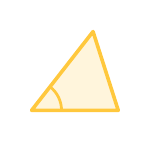
\begin{tikzpicture}[x=1cm,y=1cm]
       \useasboundingbox (-0.05,-0.05) rectangle (1.15,1.05);
       \fill[GoldAccent,opacity=.18] (0,0)--(1.1,0)--(0.78,1.0)--cycle;
       \draw[GoldAccent,line width=1.3pt,line join=round]
            (0,0)--(1.1,0)--(0.78,1.0)--cycle;
       \draw[GoldAccent,line width=1pt] (0.38,0) arc[start angle=0,end angle=52,radius=0.38];
     \end{tikzpicture}}}

% A decorative ASA triangle:  #1,#2 = lower-left corner,  #3 = TikZ line style,
% #4 = vertex-label suffix (empty or '),  #5 = label colour, #6 = coordinate prefix.
% Geometry:  A=(0,0)  B=(3.4,0)  C=(2.5,3.0)   (angles  A≈50.2°,  B≈73.3°)
\newcommand{\asatriangle}[6]{%
  \begin{scope}[shift={(#1,#2)},scale=0.72]
    \pgfmathsetmacro{\angA}{atan2(3.0,2.5)}
    \pgfmathsetmacro{\angB}{180-atan2(3.0,0.9)}
    \coordinate (#6A) at (0,0);
    \coordinate (#6B) at (3.4,0);
    \coordinate (#6C) at (2.5,3.0);
    % translucent body, then the outline; arcs/ticks use fill=none so that the
    % open arcs are not closed into filled wedges
    \path[#3,fill opacity=.14] (0,0)--(3.4,0)--(2.5,3.0)--cycle;
    \draw[#3,fill=none,line width=1.6pt,line join=round] (0,0)--(3.4,0)--(2.5,3.0)--cycle;
    % one arc at A
    \draw[#3,fill=none,solid,line width=1.1pt] (0.65,0) arc[start angle=0,end angle=\angA,radius=0.65];
    % two arcs at B (well separated so they read as a double mark)
    \draw[#3,fill=none,solid,line width=1.1pt] ($(3.4,0)+(180:0.46)$) arc[start angle=180,end angle=\angB,radius=0.46];
    \draw[#3,fill=none,solid,line width=1.1pt] ($(3.4,0)+(180:0.72)$) arc[start angle=180,end angle=\angB,radius=0.72];
    % one tick on the side AB
    \draw[#3,fill=none,solid,line width=1.3pt] (1.7,-0.12)--(1.7,0.12);
    % vertex labels (positioned so dashed translation lines do not collide with labels)
    \ifx\relax#4\relax
      \node[text=#5,font=\bfseries\itshape\fontsize{12}{14}\selectfont,anchor=south east,inner sep=2pt] at (-0.04,0.08) {$A$};
      \node[text=#5,font=\bfseries\itshape\fontsize{12}{14}\selectfont,anchor=north,inner sep=2pt] at (3.38,-0.04) {$B$};
      \node[text=#5,font=\bfseries\itshape\fontsize{12}{14}\selectfont,anchor=south,inner sep=3pt] at (2.5,3.02) {$C$};
    \else
      \node[text=#5,font=\bfseries\itshape\fontsize{12}{14}\selectfont,anchor=north east,inner sep=2pt] at (-0.02,-0.04) {$A#4$};
      \node[text=#5,font=\bfseries\itshape\fontsize{12}{14}\selectfont,anchor=north,inner sep=2pt] at (3.38,-0.04) {$B#4$};
      \node[text=#5,font=\bfseries\itshape\fontsize{12}{14}\selectfont,anchor=south east,inner sep=2pt] at (2.42,3.04) {$C#4$};
    \fi
  \end{scope}}

  \newcommand{\hwtri}[7]{%
    \begin{scope}[shift={(#1,5.0)}]
      \coordinate (#6a) at (0,0);
      \coordinate (#6b) at (3.2,0);
      \coordinate (#6c) at (#2:2.4);
      \path[draw=NavyDeep,fill=NavyDeep!4,line width=1.3pt,line join=round] (#6a)--(#6b)--(#6c)--cycle;
      \draw[NavyDeep,line width=1.3pt] (1.6,-0.13)--(1.6,0.13);
      \coordinate (#6m) at ($(#6a)!0.5!(#6c)$);
      \draw[NavyDeep,line width=1.3pt] ($(#6m)!0.07cm!(#6a)$)++(#2+90:0.12) -- ++(#2-90:0.24);
      \draw[NavyDeep,line width=1.3pt] ($(#6m)!0.07cm!(#6c)$)++(#2+90:0.12) -- ++(#2-90:0.24);
      \draw[RoyalBlue,line width=1.1pt] (0.6,0) arc[start angle=0,end angle=#2,radius=0.6];
      \node[anchor=north east,text=NavyDeep,font=\bfseries\itshape,inner sep=2pt] at (#6a) {$#3$};
      \node[anchor=north west,text=NavyDeep,font=\bfseries\itshape,inner sep=2pt] at (#6b) {$#4$};
      \node[anchor=south,text=NavyDeep,font=\bfseries\itshape,inner sep=2pt] at (#6c) {$#5$};
      \node[anchor=north,text=NavyDeep,inner sep=2pt] at (1.6,-0.12) {\fontsize{9}{11}\selectfont $5\text{ cm}$};
      \node[anchor=south east,text=NavyDeep,inner sep=2pt] at ($(#6m)+(#2+90:0.12)$) {\fontsize{9}{11}\selectfont $4\text{ cm}$};
      \node[anchor=south west,text=RoyalBlue,inner sep=1pt] at (#2/2:0.68) {\fontsize{9}{11}\selectfont $#2^\circ$};
      \node[fill=NavyDeep!6,draw=NavyDeep!25,line width=0.6pt,rounded corners=4pt,
            inner xsep=8pt,inner ysep=2.5pt,text=NavyDeep] at (3.1,2.3) {\fontsize{10}{12}\selectfont\bfseries $\Delta #3#4#5$};
      \only<4->{\draw[GreenAccent!80!black,line width=2pt] (#6a)--(#6b);}
      \only<5->{\draw[GreenAccent!80!black,line width=2pt] (#6a)--(#6c);}
      \only<6->{\draw[RedAccent,line width=1.8pt] (0.6,0) arc[start angle=0,end angle=#2,radius=0.6];}
    \end{scope}}

% ---------------------------------------------------------------------------
%  Alternate-interior-angle figure (slides 4 & 5)
%  d1 (top) and d2 (bottom) are parallel, transversal Delta cuts them at A, B.
%  Delta slopes at 60° so that  A1 (lower-left at A) = B1 (upper-right at B) = 60°
%  and A2 (lower-right at A) = B2 (upper-left at B) = 120°.
% ---------------------------------------------------------------------------
\newcommand{\altbase}{%
  \coordinate (A) at (9.0,6.0);
  \coordinate (B) at (7.268,3.0);
  % parallel lines with direction arrows
  \draw[NavyDeep,line width=1.6pt,-stealth] (3.2,6.0)--(13.0,6.0);
  \draw[NavyDeep,line width=1.6pt,-stealth] (3.2,3.0)--(13.0,3.0);
  \node[text=NavyDeep,anchor=west,font=\itshape\fontsize{13}{15}\selectfont] at (13.15,6.0) {$d_1$};
  \node[text=NavyDeep,anchor=west,font=\itshape\fontsize{13}{15}\selectfont] at (13.15,3.0) {$d_2$};
  % transversal
  \draw[NavyDeep,line width=1.6pt] ($(A)+(60:1.2)$)--($(B)+(240:1.2)$);
  \node[text=NavyDeep,anchor=south west,font=\fontsize{13}{15}\selectfont] at ($(A)+(60:1.2)$) {$\Delta$};
  % points
  \fill[NavyDeep] (A) circle (2.8pt);
  \fill[NavyDeep] (B) circle (2.8pt);
  \node[text=NavyDeep,font=\bfseries\itshape\fontsize{13}{15}\selectfont] at ($(A)+(135:0.4)$) {$A$};
  \node[text=NavyDeep,font=\bfseries\itshape\fontsize{13}{15}\selectfont] at ($(B)+(-60:0.4)$) {$B$};}

% Angle mark: #1 vertex, #2 start°, #3 end°, #4 radius, #5 colour,
%             #6 number of equal-ticks (0,1,2), #7 label, #8 label radius
\newcommand{\angmark}[8]{%
  \fill[#5,opacity=.16] (#1)--++(#2:#4) arc[start angle=#2,end angle=#3,radius=#4]--cycle;
  \draw[#5,line width=1.5pt] ($(#1)+(#2:#4)$) arc[start angle=#2,end angle=#3,radius=#4];
  \pgfmathsetmacro{\tmpmid}{(#2+#3)/2}
  \pgfmathsetmacro{\tmprl}{#4-0.1}
  \pgfmathsetmacro{\tmprh}{#4+0.1}
  \ifnum#6=1
    \draw[#5,line width=1.3pt] ($(#1)+(\tmpmid:\tmprl)$)--($(#1)+(\tmpmid:\tmprh)$);
  \fi
  \ifnum#6=2
    \pgfmathsetmacro{\tmpma}{\tmpmid-5}
    \pgfmathsetmacro{\tmpmb}{\tmpmid+5}
    \draw[#5,line width=1.3pt] ($(#1)+(\tmpma:\tmprl)$)--($(#1)+(\tmpma:\tmprh)$);
    \draw[#5,line width=1.3pt] ($(#1)+(\tmpmb:\tmprl)$)--($(#1)+(\tmpmb:\tmprh)$);
  \fi
  \node[text=#5!75!black,font=\bfseries\fontsize{10}{12}\selectfont,inner sep=0pt] at ($(#1)+(\tmpmid:#8)$) {#7};}

% thin variant (slide 19)
\newcommand{\angmarkT}[8]{%
  \fill[#5,opacity=.16] (#1)--++(#2:#4) arc[start angle=#2,end angle=#3,radius=#4]--cycle;
  \draw[#5,line width=0.8pt] ($(#1)+(#2:#4)$) arc[start angle=#2,end angle=#3,radius=#4];
  \pgfmathsetmacro{\tmpmid}{(#2+#3)/2}
  \pgfmathsetmacro{\tmprl}{#4-0.1}
  \pgfmathsetmacro{\tmprh}{#4+0.1}
  \ifnum#6=1
    \draw[#5,line width=0.7pt] ($(#1)+(\tmpmid:\tmprl)$)--($(#1)+(\tmpmid:\tmprh)$);
  \fi
  \ifnum#6=2
    \pgfmathsetmacro{\tmpma}{\tmpmid-5}
    \pgfmathsetmacro{\tmpmb}{\tmpmid+5}
    \draw[#5,line width=0.7pt] ($(#1)+(\tmpma:\tmprl)$)--($(#1)+(\tmpma:\tmprh)$);
    \draw[#5,line width=0.7pt] ($(#1)+(\tmpmb:\tmprl)$)--($(#1)+(\tmpmb:\tmprh)$);
  \fi
  \node[text=#5!75!black,font=\bfseries\fontsize{10}{12}\selectfont,inner sep=0pt] at ($(#1)+(\tmpmid:#8)$) {#7};}

% Khmer callout: #1 node name, #2 label position, #3 arrow target, #4 colour
\newcommand{\callout}[4]{%
  \node[name=#1,fill=#4!8,draw=#4,line width=0.9pt,rounded corners=4pt,
        inner xsep=8pt,inner ysep=4pt,text=#4!70!black] at (#2)
       {\fontsize{11}{14}\selectfont\bfseries មុំឆ្លាស់ក្នុង};
  \draw[#4,line width=1.1pt,-stealth,shorten >=1pt] (#1)--(#3);}

\colorlet{PairOne}{RoyalBlue}
\colorlet{PairTwo}{orange!90!black}

% ---------------------------------------------------------------------------
%  Shared pieces for slides 7 – 11
% ---------------------------------------------------------------------------
\colorlet{SideCol}{orange!90!black}   % colour for "ជ្រុង" (side)
\colorlet{AngCol}{RoyalBlue}          % colour for "មុំ"   (angle)
\colorlet{VertCol}{green!55!black}    % vertical angles
\colorlet{AdjCol}{RoyalBlue}
\colorlet{OppCol}{RedAccent}

% header / footer used by every white content slide
\newcommand{\sHdr}[2]{%
  \fill[white] (0,0) rectangle (16,9);
  \node[anchor=west,text=NavyDeep] at (0.8,8.35)
       {{\fontsize{12}{17}\selectfont\muol{#1}}\ \ |\ \ {\fontsize{10.5}{15}\selectfont\bfseries #2}};
  \draw[NavyDeep!18,line width=0.6pt] (0.8,7.98)--(15.2,7.98);}

\newcommand{\sFtr}{%
  \fill[NavyDeep] (0,0) rectangle (16,0.65);
  \shade[shading=axis,left color=GoldAccent,right color=GoldAccent!0] (0,0.65) rectangle (16,0.71);
  \node[anchor=west,inner sep=0,text=white] at (0.8,0.28)
       {\fontsize{8.5}{11}\selectfont \TeacherName\ \ |\ \ \color{SkyLight}គណិតវិទ្យា ថ្នាក់ទី៨};
  \node[anchor=east,inner sep=0,text=GoldAccent] at (15.2,0.28)
       {\fontsize{8.5}{11}\selectfont\muol{មេរៀនទី១២}\ \ \color{white}ការប្រៀបធៀបត្រីកោណ};}

% round badge: #1 x, #2 y, #3 label, #4 colour
\newcommand{\badge}[4]{%
  \fill[#4] (#1,#2) circle (0.27);
  \node[font=\bfseries\fontsize{11}{13}\selectfont,text=white,inner sep=0] at (#1,#2) {#3};}

% proof row: #1 x0, #2 y, #3 badge, #4 badge colour, #5 equation, #6 reason
\newcommand{\prow}[6]{%
  \badge{#1}{#2}{#3}{#4}
  \node[anchor=west,text=NavyDeep,inner sep=0] at (#1+0.55,#2) {\fontsize{15}{18}\selectfont #5};
  \node[anchor=west,text=black!65,inner sep=0] at (#1+5.0,#2) {\fontsize{10.5}{14}\selectfont #6};}

% gold conclusion box: #1 x, #2 y, #3 text
\newcommand{\concl}[3]{%
  \node[draw=GoldAccent!70!black,fill=GoldAccent!12,line width=0.9pt,rounded corners=6pt,
        inner xsep=16pt,inner ysep=7pt,text=NavyDeep] at (#1,#2)
       {\fontsize{13}{17}\selectfont\bfseries #3};}

% ---------------------------------------------------------------------------
%  ASA triangle  A(0,0) B(4k,0) C(2.1751k,2.1751k)   ∠A = 45°, ∠B = 50°, AB = 4 cm·k/1
%  #1 x  #2 y  #3 k  #4 colour  #5 coordinate prefix  #6 line width
% ---------------------------------------------------------------------------
\newcommand{\asaT}[6]{%
  \pgfmathsetmacro{\asaW}{4*#3}
  \pgfmathsetmacro{\asaH}{2.1751*#3}
  \coordinate (#5A) at (#1,#2);
  \coordinate (#5B) at ($(#1,#2)+(\asaW,0)$);
  \coordinate (#5C) at ($(#1,#2)+(\asaH,\asaH)$);
  \path[fill=#4,fill opacity=.12] (#5A)--(#5B)--(#5C)--cycle;
  \draw[#4,line width=#6,line join=round] (#5A)--(#5B)--(#5C)--cycle;
  \draw[#4,line width=1.1pt] ($(#5A)+(0.75,0)$) arc[start angle=0,end angle=45,radius=0.75];
  \draw[#4,line width=1.1pt] ($(#5B)+(180:0.5)$) arc[start angle=180,end angle=130,radius=0.5];
  \draw[#4,line width=1.1pt] ($(#5B)+(180:0.72)$) arc[start angle=180,end angle=130,radius=0.72];
  \draw[#4,line width=1.4pt] ($(#5A)!0.5!(#5B)+(0,-0.12)$)--++(0,0.24);}

% unfilled variant of \asaT
\newcommand{\asaTn}[6]{%
  \pgfmathsetmacro{\asaW}{4*#3}
  \pgfmathsetmacro{\asaH}{2.1751*#3}
  \coordinate (#5A) at (#1,#2);
  \coordinate (#5B) at ($(#1,#2)+(\asaW,0)$);
  \coordinate (#5C) at ($(#1,#2)+(\asaH,\asaH)$);
  \draw[#4,line width=#6,line join=round] (#5A)--(#5B)--(#5C)--cycle;
  \draw[#4,line width=1.1pt] ($(#5A)+(0.75,0)$) arc[start angle=0,end angle=45,radius=0.75];
  \draw[#4,line width=1.1pt] ($(#5B)+(180:0.5)$) arc[start angle=180,end angle=130,radius=0.5];
  \draw[#4,line width=1.1pt] ($(#5B)+(180:0.72)$) arc[start angle=180,end angle=130,radius=0.72];
  \draw[#4,line width=1.4pt] ($(#5A)!0.5!(#5B)+(0,-0.12)$)--++(0,0.24);}

% vertex labels: #1 prefix  #2 suffix ('' or empty)  #3 colour
\newcommand{\asaL}[3]{%
  \node[text=#3,font=\bfseries\itshape\fontsize{13}{15}\selectfont,anchor=north east,inner sep=2pt] at (#1A) {$A#2$};
  \node[text=#3,font=\bfseries\itshape\fontsize{13}{15}\selectfont,anchor=north west,inner sep=2pt] at (#1B) {$B#2$};
  \node[text=#3,font=\bfseries\itshape\fontsize{13}{15}\selectfont,anchor=south,inner sep=3pt] at (#1C) {$C#2$};}

% measurements: #1 prefix  #2 colour
\newcommand{\asaV}[2]{%
  \node[text=#2,font=\bfseries\fontsize{9.5}{11}\selectfont,inner sep=0] at ($(#1A)+(22.5:1.15)$) {$45^\circ$};
  \node[text=#2,font=\bfseries\fontsize{9.5}{11}\selectfont,inner sep=0] at ($(#1B)+(155:1.28)$) {$50^\circ$};
  \node[text=#2,font=\bfseries\fontsize{10.5}{12}\selectfont,anchor=north,inner sep=1pt] at ($(#1A)!0.5!(#1B)+(0,-0.16)$) {$4\text{ cm}$};}

% "the three remaining elements" AC, BC, ∠C : #1 prefix
\newcommand{\asaQ}[1]{%
  \draw[RedAccent,line width=2.8pt,dash pattern=on 5pt off 3pt] (#1A)--(#1C)--(#1B);
  \draw[RedAccent,line width=1.7pt] ($(#1C)+(225:0.55)$) arc[start angle=225,end angle=310,radius=0.55];
  \node[text=RedAccent,font=\bfseries\fontsize{14}{16}\selectfont,inner sep=0] at ($(#1C)+(267:0.95)$) {?};
  \node[text=RedAccent,font=\bfseries\fontsize{14}{16}\selectfont,inner sep=0] at ($(#1A)!0.5!(#1C)+(135:0.32)$) {?};
  \node[text=RedAccent,font=\bfseries\fontsize{14}{16}\selectfont,inner sep=0] at ($(#1B)!0.5!(#1C)+(45:0.32)$) {?};}

% moving copy of ΔA'B'C' for the superposition animation: #1 frame, #2 fraction of travel left
\newcommand{\movetri}[3]{%
  \only<#1>{%
    \pgfmathsetmacro{\mdx}{8.4*#2}
    \pgfmathsetmacro{\mdy}{0.45*#2}
    \asaT{1.9+\mdx}{2.9+\mdy}{1.2}{orange!90!black}{m}{1.8pt}
    \ifnum#3=1 \asaL{m}{'}{orange!85!black}\asaV{m}{orange!85!black}\fi}}

% ---------------------------------------------------------------------------
%  Model problem figure (slide 9):  AB and CD cross at E, AD ∥ CB, EA = EB
%  #1,#2 position of E   #3 scale
% ---------------------------------------------------------------------------
\newcommand{\modelfig}[3]{%
  \coordinate (E) at (#1,#2);
  \coordinate (A) at ($(E)+(-2.4*#3,1.3*#3)$);
  \coordinate (D) at ($(E)+(1.5*#3,1.3*#3)$);
  \coordinate (B) at ($(E)+(2.4*#3,-1.3*#3)$);
  \coordinate (C) at ($(E)+(-1.5*#3,-1.3*#3)$);}
\newcommand{\modelbase}{%
  \draw[NavyDeep,line width=1.8pt,line join=round] (A)--(B) (C)--(D) (A)--(D) (C)--(B);
  \fill[NavyDeep] (A) circle (2.4pt) (B) circle (2.4pt) (C) circle (2.4pt) (D) circle (2.4pt) (E) circle (2.4pt);
  \foreach \p/\an/\nm in {A/south east/A,B/north west/B,C/north east/C,D/south west/D}{
    \node[text=NavyDeep,font=\bfseries\itshape\fontsize{13}{15}\selectfont,anchor=\an,inner sep=3pt] at (\p) {$\nm$};}
  \node[text=NavyDeep,font=\bfseries\itshape\fontsize{13}{15}\selectfont,anchor=north,inner sep=7pt] at (E) {$E$};}
\newcommand{\mSides}[1]{%
  \draw[#1,line width=2.2pt] ($(A)!0.5!(E)$)++(61.56:0.13)--++(241.56:0.26);
  \draw[#1,line width=2.2pt] ($(B)!0.5!(E)$)++(61.56:0.13)--++(241.56:0.26);}
\newcommand{\mPar}[1]{%
  \draw[#1,line width=1.9pt,line cap=round,line join=round] ($(A)!0.5!(D)+(-0.07,0.11)$)--++(0.14,-0.11)--++(-0.14,-0.11);
  \draw[#1,line width=1.9pt,line cap=round,line join=round] ($(C)!0.5!(B)+(-0.07,0.11)$)--++(0.14,-0.11)--++(-0.14,-0.11);}
\newcommand{\mVert}[2]{%
  \angmark{E}{40.9}{151.6}{#2}{#1}{2}{}{0}
  \angmark{E}{220.9}{331.6}{#2}{#1}{2}{}{0}}
\newcommand{\mAlt}[2]{%
  \angmark{A}{-28.44}{0}{#2}{#1}{1}{}{0}
  \angmark{B}{151.56}{180}{#2}{#1}{1}{}{0}}

% ---------------------------------------------------------------------------
%  Practice figure (slide 10): B on AD, E on AC, AB = AE, AD = AC
%  #1,#2 position of A   #3 = AB = AE   #4 = AD = AC   (ratio 1 : 2 !)
% ---------------------------------------------------------------------------
\newcommand{\tenfig}[4]{%
  \coordinate (A) at (#1,#2);
  \coordinate (B) at ($(A)+(32:#3)$);
  \coordinate (D) at ($(A)+(32:#4)$);
  \coordinate (E) at ($(A)+(-24:#3)$);
  \coordinate (C) at ($(A)+(-24:#4)$);}
\newcommand{\tenbase}{%
  \draw[NavyDeep,line width=0.9pt,line join=round] (A)--(D) (A)--(C) (B)--(C) (E)--(D);
  \fill[NavyDeep] (A) circle (1.8pt) (B) circle (1.8pt) (C) circle (1.8pt) (D) circle (1.8pt) (E) circle (1.8pt);
  \node[text=NavyDeep,font=\bfseries\itshape\fontsize{13}{15}\selectfont,anchor=east,inner sep=4pt] at (A) {$A$};
  \node[text=NavyDeep,font=\bfseries\itshape\fontsize{13}{15}\selectfont,inner sep=0] at ($(B)+(122:0.33)$) {$B$};
  \node[text=NavyDeep,font=\bfseries\itshape\fontsize{13}{15}\selectfont,inner sep=0] at ($(E)+(-114:0.33)$) {$E$};
  \node[text=NavyDeep,font=\bfseries\itshape\fontsize{13}{15}\selectfont,anchor=south west,inner sep=3pt] at (D) {$D$};
  \node[text=NavyDeep,font=\bfseries\itshape\fontsize{13}{15}\selectfont,anchor=north west,inner sep=3pt] at (C) {$C$};}
\newcommand{\tSides}[1]{%
  \draw[#1,line width=0.7pt] ($(A)!0.5!(B)$)++(122:0.13)--++(302:0.26);
  \draw[#1,line width=0.7pt] ($(A)!0.5!(E)$)++(66:0.13)--++(246:0.26);}
\newcommand{\tAngBE}[2]{%
  \angmarkT{B}{212}{306.1}{#2}{#1}{2}{}{0}
  \angmarkT{E}{61.9}{156}{#2}{#1}{2}{}{0}}
\newcommand{\tAngA}[2]{%
  \angmarkT{A}{-24}{32}{#2}{#1}{1}{}{0}}

% ---------------------------------------------------------------------------
%  Homework figure (slide 11):  #1,#2 = position of the origin   #3 = scale
% ---------------------------------------------------------------------------
\newcommand{\homefig}[3]{%
  \coordinate (B) at ($(#1,#2)+(2.6*#3,0)$);
  \coordinate (C) at ($(#1,#2)+(7.0*#3,0)$);
  \coordinate (A) at ($(#1,#2)+(4.2*#3,5.0*#3)$);
  \coordinate (D) at ($(#1,#2)+(4.70366*#3,0)$);
  \coordinate (E) at ($(#1,#2)+(6.76505*#3,0.41955*#3)$);
  \coordinate (K) at ($(#1,#2)+(2.45345*#3,-0.45798*#3)$);}
\newcommand{\hnode}[3]{% point, anchor, label
  \node[text=NavyDeep,font=\bfseries\itshape\fontsize{13}{15}\selectfont,anchor=#2,inner sep=3pt] at (#1) {$#3$};}
\newcommand{\hometri}{%
  \draw[NavyDeep,line width=1.8pt,line join=round] (A)--(B)--(C)--cycle;
  \fill[NavyDeep] (A) circle (2.4pt) (B) circle (2.4pt) (C) circle (2.4pt);
  \hnode{A}{south}{A}\hnode{B}{east}{B}\hnode{C}{north west}{C}}
\newcommand{\homebis}{%
  \draw[NavyDeep,line width=1.8pt] (A)--(D);
  \fill[NavyDeep] (D) circle (2.4pt);
  \hnode{D}{north}{D}
  \angmark{A}{-107.74}{-84.25}{0.8}{AngCol}{1}{}{0}
  \angmark{A}{-84.25}{-60.75}{0.8}{AngCol}{1}{}{0}}
\newcommand{\homeE}{%
  \draw[NavyDeep,line width=1.8pt] (E)--(D);
  \fill[NavyDeep] (E) circle (2.4pt);
  \hnode{E}{south west}{E}
  \angmark{D}{95.75}{180}{0.62}{SideCol}{2}{}{0}
  \angmark{D}{11.50}{95.75}{0.62}{SideCol}{2}{}{0}}
\newcommand{\homeK}{%
  \draw[NavyDeep,line width=1.8pt] (D)--(K);
  \draw[NavyDeep,line width=1.8pt,dash pattern=on 5pt off 4pt] (B)--(K);
  \fill[NavyDeep] (K) circle (2.4pt);
  \hnode{K}{north}{K}}

% ---------------------------------------------------------------------------
%  Global bold maths: every formula is bold, and math is set ~8% smaller so
%  the bold glyphs keep the same footprint as the old light ones.
% ---------------------------------------------------------------------------
\AtBeginDocument{\mathversion{bold}}
\DeclareMathSizes{3.8}{3.5}{2.52}{1.82}
\DeclareMathSizes{4.6}{4.23}{3.05}{2.2}
\DeclareMathSizes{5.5}{5.06}{3.64}{2.63}
\DeclareMathSizes{7}{6.44}{4.64}{3.35}
\DeclareMathSizes{8}{7.36}{5.3}{3.83}
\DeclareMathSizes{8.5}{7.82}{5.63}{4.07}
\DeclareMathSizes{9}{8.28}{5.96}{4.31}
\DeclareMathSizes{9.5}{8.74}{6.29}{4.54}
\DeclareMathSizes{10}{9.2}{6.62}{4.78}
\DeclareMathSizes{10.5}{9.66}{6.96}{5.02}
\DeclareMathSizes{10.95}{10.07}{7.25}{5.24}
\DeclareMathSizes{11}{10.12}{7.29}{5.26}
\DeclareMathSizes{11.5}{10.58}{7.62}{5.5}
\DeclareMathSizes{12}{11.04}{7.95}{5.74}
\DeclareMathSizes{12.5}{11.5}{8.28}{5.98}
\DeclareMathSizes{13}{11.96}{8.61}{6.22}
\DeclareMathSizes{13.5}{12.42}{8.94}{6.46}
\DeclareMathSizes{14}{12.88}{9.27}{6.7}
\DeclareMathSizes{14.4}{13.25}{9.54}{6.89}
\DeclareMathSizes{14.5}{13.34}{9.6}{6.94}
\DeclareMathSizes{15}{13.8}{9.94}{7.18}
\DeclareMathSizes{16}{14.72}{10.6}{7.65}
\DeclareMathSizes{17}{15.64}{11.26}{8.13}
\DeclareMathSizes{17.28}{15.9}{11.45}{8.27}
\DeclareMathSizes{18}{16.56}{11.92}{8.61}
\DeclareMathSizes{18.5}{17.02}{12.25}{8.85}
\DeclareMathSizes{19}{17.48}{12.59}{9.09}
\DeclareMathSizes{20}{18.4}{13.25}{9.57}
\DeclareMathSizes{20.74}{19.08}{13.74}{9.92}
\DeclareMathSizes{22}{20.24}{14.57}{10.52}
\DeclareMathSizes{24.88}{22.89}{16.48}{11.9}
\DeclareMathSizes{26}{23.92}{17.22}{12.44}
\DeclareMathSizes{34}{31.28}{22.52}{16.27}

\begin{document}

% =============================================================================
%  SLIDE 1 – Title slide
% =============================================================================
\begin{frame}[plain]
\begin{tikzpicture}[remember picture,overlay,shift={(current page.south west)},x=1cm,y=1cm]

  % ---- background: deep navy → royal blue gradient ------------------------
  \shade[shading=axis,shading angle=-35,left color=NavyDeep,right color=RoyalBlue]
       (0,0) rectangle (16,9);

  % ---- soft geometric shapes (PowerPoint "design ideas" feel) -------------
  \fill[white,fill opacity=.055] (16,0)--(16,9)--(10.1,9)--(6.6,0)--cycle;
  \fill[white,fill opacity=.045] (16,0)--(16,9)--(12.4,9)--(10.2,0)--cycle;
  \fill[SkyLight,fill opacity=.10] (13.1,4.7) circle (3.45);
  \draw[SkyLight,opacity=.28,line width=.8pt] (13.1,4.7) circle (3.95);
  \fill[GoldAccent,fill opacity=.9] (15.12,1.1) circle (.07);
  \fill[SkyLight,fill opacity=.8] (10.0,8.1) circle (.05);
  \fill[SkyLight,fill opacity=.5] (14.9,8.3) circle (.09);

  % ---- top-left: school name ----------------------------------------------
  \node[anchor=south west,inner sep=0,text=white] at (0.95,7.95)
       {\fontsize{14}{22}\selectfont\muol{វិទ្យាល័យព្រែកលៀប (សាលារៀនជំនាន់ថ្មី)}};
  \node[anchor=south west,inner sep=0,text=SkyLight] at (0.95,7.50)
       {\fontsize{9.5}{12}\selectfont\addfontfeature{LetterSpace=10}PREAK LEAP HIGH SCHOOL (NGS)};
  \draw[white,opacity=.25,line width=.6pt] (0.95,7.12)--(10.5,7.12);

  % ---- lesson title -------------------------------------------------------
  \node[anchor=west,inner sep=0,text=GoldAccent] at (0.95,6.35)
       {\fontsize{16}{24}\selectfont\muol{មេរៀនទី១២}};
  \node[anchor=west,inner sep=0,text=white] at (0.95,4.75)
       {\fontsize{26}{38}\selectfont\muol{ការប្រៀបធៀបត្រីកោណ}};
  \node[anchor=west,inner sep=0,text=GoldAccent] at (0.95,3.15)
       {\fontsize{18}{26}\selectfont\muol{ត្រីកោណប៉ុនគ្នា (ករណី ម.ជ.ម)}};

  % ---- bottom row: teacher name (left) & subject pill (far right) ---------
  \node[anchor=west,inner sep=0]
       at (0.95,0.85)
       {{\fontsize{13}{17}\selectfont{\color{GoldAccent}\bfseries បង្រៀនដោយ\ \,}{\color{white}\muol{\TeacherName}}}};

  \node[anchor=east,fill=GoldAccent,text=NavyDeep,rounded corners=10pt,
        inner xsep=12pt,inner ysep=4pt]
       at (15.05,0.85) {\fontsize{11.5}{15}\selectfont\bfseries គណិតវិទ្យា ថ្នាក់ទី៨};

  % ---- right: two congruent triangles (ASA motif) -------------------------
  % Triangle A'B'C' (initial position, solid line, gold color)
  \asatriangle{11.55}{2.95}{draw=GoldAccent,fill=GoldAccent}{'}{GoldAccent}{Tfront}

  % Triangle ABC (destination position at the back, solid line, white color)
  \asatriangle{13.10}{3.80}{draw=white,fill=white}{}{white}{Tback}

  % Dashed connecting lines between corresponding vertices
  \draw[SkyLight, line width=1.1pt, dash pattern=on 4pt off 3.5pt] (TfrontA) -- (TbackA);
  \draw[SkyLight, line width=1.1pt, dash pattern=on 4pt off 3.5pt] (TfrontB) -- (TbackB);
  \draw[SkyLight, line width=1.1pt, dash pattern=on 4pt off 3.5pt] (TfrontC) -- (TbackC);

  % ---- bottom accent line -------------------------------------------------
  \shade[shading=axis,left color=GoldAccent,right color=GoldAccent!0] (0,0) rectangle (16,.12);

\end{tikzpicture}
\end{frame}

% =============================================================================
%  SLIDE 2 – Homework Review (Vertical triangle stack, wide solution card)
%    1: problem (header)           2: the two triangles + question
%    3: congruence rule            4: ST = DE  (side highlighted on both)
%    5: SR = DF  (side highlighted) 6: angle S ≠ angle D (arcs in red)
%    7: conclusion
% =============================================================================
\begin{frame}
\begin{tikzpicture}[remember picture,overlay,shift={(current page.south west)},x=1cm,y=1cm]

  \fill[white] (0,0) rectangle (16,9);

  % ---- header ----------------------------------------------------------------
  \node[anchor=west,text=NavyDeep] at (0.8, 8.45)
       {{\fontsize{12.5}{17}\selectfont\muol{កំណែកិច្ចការផ្ទះ}}\ \ %
        {\fontsize{10}{14}\selectfont ពន្យល់ថាតើត្រីកោណទាំងពីរខាងក្រោម ប៉ុនគ្នាឬទេ?}};
  \draw[NavyDeep!18,line width=0.6pt] (0.8,8.12)--(15.2,8.12);

  % ---- TOP: two triangles side by side, centred in each half -----------------
  % #1 = x of left vertex, #2 = angle, #3,#4,#5 = vertex names, #6 = prefix, #7 = name pill

  \only<2->{
    \hwtri{3.0}{50}{S}{T}{R}{L}{}
    \hwtri{10.0}{60}{D}{E}{F}{M}{}

    \draw[NavyDeep!14,line width=0.5pt,dashed] (8,4.5)--(8,7.7);
    \draw[NavyDeep!18,line width=0.6pt] (0.8,4.3)--(15.2,4.3);
  }

  % ---- BOTTOM: solution -------------------------------------------------------
  \only<2>{
    \node[text=NavyDeep] at (8,2.4) {%
      {\fontsize{18}{24}\selectfont តើត្រីកោណទាំងពីរនេះ\ \color{RoyalBlue}\bfseries ប៉ុនគ្នាដែរឬទេ?}};
  }

  \only<3->{
    \node[anchor=west,font=\bfseries,text=NavyDeep] at (0.8,3.95)
         {\fontsize{11}{16}\selectfont គេដឹងថា ត្រីកោណពីរប៉ុនគ្នា លុះត្រាតែធាតុត្រូវគ្នាជាធាតុប៉ុនគ្នា};
  }
  \only<4->{
    \fill[GreenAccent!20] (1.15,2.95) circle (6.5pt);
    \draw[GreenAccent!80!black,line width=0.9pt] (1.15,2.95) circle (6.5pt);
    \draw[GreenAccent!80!black,line width=1.2pt,line cap=round,line join=round] (1.15,2.95)++(-3pt,-0.5pt)--++(2pt,-2pt)--++(4.2pt,5pt);
    \node[anchor=west,text=NavyDeep] at (1.6,2.95) {%
      {\fontsize{14}{18}\selectfont $\boldsymbol{ST = DE}$}\ \ {\fontsize{11}{16}\selectfont\color{black!70}(ជ្រុងត្រូវគ្នាប៉ុនគ្នា)}};
  }
  \only<5->{
    \fill[GreenAccent!20] (1.15,2.15) circle (6.5pt);
    \draw[GreenAccent!80!black,line width=0.9pt] (1.15,2.15) circle (6.5pt);
    \draw[GreenAccent!80!black,line width=1.2pt,line cap=round,line join=round] (1.15,2.15)++(-3pt,-0.5pt)--++(2pt,-2pt)--++(4.2pt,5pt);
    \node[anchor=west,text=NavyDeep] at (1.6,2.15) {%
      {\fontsize{14}{18}\selectfont $\boldsymbol{SR = DF}$}\ \ {\fontsize{11}{16}\selectfont\color{black!70}(ជ្រុងត្រូវគ្នាប៉ុនគ្នា)}};
  }
  \only<6->{
    \fill[RedAccent!15] (1.15,1.35) circle (6.5pt);
    \draw[RedAccent!80!black,line width=0.9pt] (1.15,1.35) circle (6.5pt);
    \draw[RedAccent!80!black,line width=1.2pt,line cap=round] (1.15,1.35)++(-2.2pt,-2.2pt)--++(4.4pt,4.4pt);
    \draw[RedAccent!80!black,line width=1.2pt,line cap=round] (1.15,1.35)++(-2.2pt,2.2pt)--++(4.4pt,-4.4pt);
    \node[anchor=west,text=NavyDeep] at (1.6,1.35) {%
      {\fontsize{14}{18}\selectfont $\boldsymbol{\angle S \neq \angle D}$}\ \ {\fontsize{11}{16}\selectfont\color{RedAccent!85!black}(មុំត្រូវគ្នាមិនប៉ុនគ្នា)}};
  }
  \only<7->{
    \fill[RedAccent!6] (9.8,1.0) rectangle (15.2,3.5);
    \draw[RedAccent!50,line width=0.8pt] (9.8,1.0) rectangle (15.2,3.5);
    \node[anchor=west,text=RoyalBlue] at (10.1,3.0) {\fontsize{12}{16}\selectfont\muol{សន្និដ្ឋាន}};
    \node[anchor=west,text=NavyDeep,font=\bfseries] at (10.1,2.25)
         {\fontsize{11.5}{16}\selectfont ត្រីកោណទាំងពីរ\ \textcolor{RedAccent!90!black}{\textbf{មិនប៉ុនគ្នាទេ}}};
    \node[anchor=west,text=black!80] at (10.1,1.5)
         {\fontsize{12}{16}\selectfont $\boldsymbol{\Delta STR \not\cong \Delta DEF}$};
  }

  % ---- footer ----------------------------------------------------------------
  \fill[NavyDeep] (0,0) rectangle (16,0.65);
  \shade[shading=axis,left color=GoldAccent,right color=GoldAccent!0] (0,0.65) rectangle (16,0.71);
  \node[anchor=west,inner sep=0,text=white] at (0.8,0.28)
       {\fontsize{8.5}{11}\selectfont \TeacherName\ \ |\ \ \color{SkyLight}គណិតវិទ្យា ថ្នាក់ទី៨};
  \node[anchor=east,inner sep=0,text=GoldAccent] at (15.2,0.28)
       {\fontsize{8.5}{11}\selectfont\muol{មេរៀនទី១២}\ \ \color{white}ការប្រៀបធៀបត្រីកោណ};

\end{tikzpicture}
\end{frame}

% =============================================================================
%  SLIDE 3 – Angle Construction with Protractor (5 Steps Animation, 7 frames)
%    1: title only   2: step 1   3: step 2   4-5: step 3   6: step 4   7: step 5
% =============================================================================
\begin{frame}
\begin{tikzpicture}[remember picture,overlay,shift={(current page.south west)},x=1cm,y=1cm]

  \fill[white] (0,0) rectangle (16,9);

  % ---- header ----------------------------------------------------------------
  \node[anchor=west,text=NavyDeep] at (0.8, 8.35)
       {{\fontsize{12}{17}\selectfont\muol{រំលឹកមេរៀន}}\ \ |\ \ %
        {\fontsize{10.5}{15}\selectfont\bfseries របៀបសង់មុំដោយប្រើរ៉ាប់ទ័រ}};
  \draw[NavyDeep!18,line width=0.6pt] (0.8,7.98)--(15.2,7.98);

  % ---- vertical separator between steps panel and canvas (from frame 2) --------------------
  \draw<2->[NavyDeep!12,line width=0.5pt,dashed] (6.65,0.7)--(6.65,7.85);

  % ---- LEFT PANEL: 5 STEPS (x from 0.55 to 6.45, width = 5.90cm) -------------
  % Frame 1 = title only.  Each card is revealed on its own frame (active look),
  % then settles to the quiet "done" look when the next step arrives.
  % Step 1 card (y: 6.48 to 7.74, center y = 7.11)         active <2>   done <3->
  \fill<2>[RoyalBlue!8,rounded corners=5pt] (0.55,6.48) rectangle (6.45,7.74);
  \draw<2>[RoyalBlue,line width=1pt,rounded corners=5pt] (0.55,6.48) rectangle (6.45,7.74);
  \fill<3->[NavyDeep!3,rounded corners=5pt] (0.55,6.48) rectangle (6.45,7.74);
  \draw<3->[NavyDeep!15,line width=0.5pt,rounded corners=5pt] (0.55,6.48) rectangle (6.45,7.74);

  \fill<2>[GoldAccent] (1.02,7.11) circle (6.5pt);
  \node<2>[font=\bfseries\fontsize{8.5}{10}\selectfont,text=NavyDeep] at (1.02,7.11) {១};
  \fill<3->[RoyalBlue!15] (1.02,7.11) circle (6.5pt);
  \draw<3->[RoyalBlue!70,line width=0.8pt] (1.02,7.11) circle (6.5pt);
  \node<3->[font=\bfseries\fontsize{8.5}{10}\selectfont,text=RoyalBlue!80!black] at (1.02,7.11) {១};
  \node<2>[anchor=west,inner sep=0,text=StepNavy] at (1.42,7.11) {%
    {\fontsize{9}{12}\selectfont\bfseries គូសកន្លះបន្ទាត់ដើម $OA$}};
  \node<3->[anchor=west,inner sep=0,text=black!75] at (1.42,7.11) {%
    {\fontsize{9}{12}\selectfont គូសកន្លះបន្ទាត់ដើម $OA$}};

  % Step 2 card (y: 5.10 to 6.36, center y = 5.73)         active <3>   done <4->
  \fill<3>[RoyalBlue!8,rounded corners=5pt] (0.55,5.10) rectangle (6.45,6.36);
  \draw<3>[RoyalBlue,line width=1pt,rounded corners=5pt] (0.55,5.10) rectangle (6.45,6.36);
  \fill<4->[NavyDeep!3,rounded corners=5pt] (0.55,5.10) rectangle (6.45,6.36);
  \draw<4->[NavyDeep!15,line width=0.5pt,rounded corners=5pt] (0.55,5.10) rectangle (6.45,6.36);

  \fill<3>[GoldAccent] (1.02,5.73) circle (6.5pt);
  \node<3>[font=\bfseries\fontsize{8.5}{10}\selectfont,text=NavyDeep] at (1.02,5.73) {២};
  \fill<4->[RoyalBlue!15] (1.02,5.73) circle (6.5pt);
  \draw<4->[RoyalBlue!70,line width=0.8pt] (1.02,5.73) circle (6.5pt);
  \node<4->[font=\bfseries\fontsize{8.5}{10}\selectfont,text=RoyalBlue!80!black] at (1.02,5.73) {២};
  \node<3>[anchor=west,inner sep=0,text=StepNavy] at (1.42,5.73) {%
    {\fontsize{8.5}{11.5}\selectfont\bfseries ដាក់ផ្ចិតរ៉ាប់ទ័រចំ $O$ និងបាតលើ $OA$}};
  \node<4->[anchor=west,inner sep=0,text=black!75] at (1.42,5.73) {%
    {\fontsize{8.5}{11.5}\selectfont ដាក់ផ្ចិតរ៉ាប់ទ័រចំ $O$ និងបាតលើ $OA$}};

  % Step 3 card (y: 3.72 to 4.98, center y = 4.35)         active <4-5> done <6->
  \fill<4-5>[RoyalBlue!8,rounded corners=5pt] (0.55,3.72) rectangle (6.45,4.98);
  \draw<4-5>[RoyalBlue,line width=1pt,rounded corners=5pt] (0.55,3.72) rectangle (6.45,4.98);
  \fill<6->[NavyDeep!3,rounded corners=5pt] (0.55,3.72) rectangle (6.45,4.98);
  \draw<6->[NavyDeep!15,line width=0.5pt,rounded corners=5pt] (0.55,3.72) rectangle (6.45,4.98);

  \fill<4-5>[GoldAccent] (1.02,4.35) circle (6.5pt);
  \node<4-5>[font=\bfseries\fontsize{8.5}{10}\selectfont,text=NavyDeep] at (1.02,4.35) {៣};
  \fill<6->[RoyalBlue!15] (1.02,4.35) circle (6.5pt);
  \draw<6->[RoyalBlue!70,line width=0.8pt] (1.02,4.35) circle (6.5pt);
  \node<6->[font=\bfseries\fontsize{8.5}{10}\selectfont,text=RoyalBlue!80!black] at (1.02,4.35) {៣};
  \node<4-5>[anchor=west,inner sep=0,text=StepNavy] at (1.42,4.35) {%
    {\fontsize{8.5}{11.5}\selectfont\bfseries ចំណាំចំណុច $B$ ត្រង់ខ្នាត $50^\circ$}};
  \node<6->[anchor=west,inner sep=0,text=black!75] at (1.42,4.35) {%
    {\fontsize{8.5}{11.5}\selectfont ចំណាំចំណុច $B$ ត្រង់ខ្នាត $50^\circ$}};

  % Step 4 card (y: 2.34 to 3.60, center y = 2.97)         active <6>   done <7>
  \fill<6>[RoyalBlue!8,rounded corners=5pt] (0.55,2.34) rectangle (6.45,3.60);
  \draw<6>[RoyalBlue,line width=1pt,rounded corners=5pt] (0.55,2.34) rectangle (6.45,3.60);
  \fill<7>[NavyDeep!3,rounded corners=5pt] (0.55,2.34) rectangle (6.45,3.60);
  \draw<7>[NavyDeep!15,line width=0.5pt,rounded corners=5pt] (0.55,2.34) rectangle (6.45,3.60);

  \fill<6>[GoldAccent] (1.02,2.97) circle (6.5pt);
  \node<6>[font=\bfseries\fontsize{8.5}{10}\selectfont,text=NavyDeep] at (1.02,2.97) {៤};
  \fill<7>[RoyalBlue!15] (1.02,2.97) circle (6.5pt);
  \draw<7>[RoyalBlue!70,line width=0.8pt] (1.02,2.97) circle (6.5pt);
  \node<7>[font=\bfseries\fontsize{8.5}{10}\selectfont,text=RoyalBlue!80!black] at (1.02,2.97) {៤};
  \node<6>[anchor=west,inner sep=0,text=StepNavy] at (1.42,2.97) {%
    {\fontsize{8.5}{11.5}\selectfont\bfseries ដាក់បន្ទាត់តាម $O, B$ គូសកន្លះបន្ទាត់ $OB$}};
  \node<7>[anchor=west,inner sep=0,text=black!75] at (1.42,2.97) {%
    {\fontsize{8.5}{11.5}\selectfont ដាក់បន្ទាត់តាម $O, B$ គូសកន្លះបន្ទាត់ $OB$}};

  % Step 5 card (y: 0.96 to 2.22, center y = 1.59)         result <7>
  \fill<7>[RoyalBlue!6,rounded corners=5pt] (0.55,0.96) rectangle (6.45,2.22);
  \draw<7>[RoyalBlue!40,line width=1.1pt,rounded corners=5pt] (0.55,0.96) rectangle (6.45,2.22);

  \fill<7>[RoyalBlue!15] (1.02,1.59) circle (6.5pt);
  \draw<7>[RoyalBlue!70,line width=0.8pt] (1.02,1.59) circle (6.5pt);
  \node<7>[font=\bfseries\fontsize{8.5}{10}\selectfont,text=RoyalBlue!80!black] at (1.02,1.59) {៥};
  \node<7>[anchor=west,inner sep=0,text=black!75] at (1.42,1.59) {%
    {\fontsize{8.5}{11.5}\selectfont\bfseries ទទួលបានមុំ $\angle AOB = 50^\circ$}};

  % ---- RIGHT PANEL: GEOMETRIC ANIMATION CANVAS -------------------------------
  % FIXED COORDINATES (Zero-drift: elements NEVER move)
  \coordinate (O) at (10.55, 4.0);
  \coordinate (A) at ($(O)+(3.8, 0)$);
  \coordinate (B) at ($(O)+(50:3.38)$);
  \coordinate (Bend) at ($(O)+(50:3.8)$);

  % 1. BASE RAY OA (appears with step 1 = frame 2, then stays completely fixed)
  \only<2->{
    \draw[RoyalBlue,line width=1.8pt,-stealth] (O) -- (A);
    \fill[NavyDeep] (O) circle (2.4pt);
    \node[anchor=north east,font=\bfseries\itshape\fontsize{13}{15}\selectfont,text=NavyDeep] at ($(O)+(-0.06,-0.06)$) {$O$};
    \node[anchor=north,font=\bfseries\itshape\fontsize{13}{15}\selectfont,text=NavyDeep] at ($(A)+(-0.35,-0.15)$) {$A$};
  }

  % 2. PROTRACTOR (Visible in frames 3 & 4 only - Authentic Black & White drafting design)
  \only<3-4>{
    \begin{scope}[shift={(O)}]
      % Clear white acrylic body (radius 3.35cm)
      \fill[white,draw=black!85,line width=0.8pt,opacity=0.94]
           (-3.35,0) -- (3.35,0) arc[start angle=0,end angle=180,radius=3.35] -- cycle;
      % Inner clear window (radius 1.45cm)
      \fill[white,draw=black!50,line width=0.5pt,opacity=0.98]
           (-1.45,0) -- (1.45,0) arc[start angle=0,end angle=180,radius=1.45] -- cycle;

      % Baseline guideline
      \draw[black!75,line width=0.6pt] (-3.3,0) -- (3.3,0);
      % Center origin crosshair at O
      \draw[black!90,line width=0.9pt] (-0.35,0) -- (0.35,0);
      \draw[black!90,line width=0.9pt] (0,-0.08) -- (0,0.35);
      \draw[black!80,line width=0.5pt] (0,0) circle (1.2pt);
      % 90-degree central perpendicular guide
      \draw[black!35,line width=0.4pt,dashed] (0,0.4) -- (0,2.68);

      % Concentric circular guide arcs for realistic drafting look
      \draw[black!55,line width=0.4pt] (0:3.02) arc[start angle=0,end angle=180,radius=3.02];
      \draw[black!40,line width=0.35pt] (0:2.68) arc[start angle=0,end angle=180,radius=2.68];
      \draw[black!30,line width=0.3pt] (0:2.42) arc[start angle=0,end angle=180,radius=2.42];

      % 1° Minor ticks (every 1° from 0° to 180°)
      \foreach \ang in {0,1,...,180} {
        \draw[black!65,line width=0.2pt] (\ang:3.24) -- (\ang:3.35);
      }
      % 5° Medium ticks (every 5° from 0° to 180°)
      \foreach \ang in {0,5,...,180} {
        \draw[black!85,line width=0.38pt] (\ang:3.15) -- (\ang:3.35);
      }
      % 10° Major ticks (every 10° from 0° to 180°)
      \foreach \ang in {0,10,...,180} {
        \draw[black,line width=0.65pt] (\ang:3.02) -- (\ang:3.35);
      }

      % Outer scale numbers (0 to 180 counter-clockwise, NO degree sign!)
      \foreach \ang in {0,10,...,180} {
        \ifnum\ang=0 \def\lblshift{3.5pt}\else\ifnum\ang=180 \def\lblshift{3.5pt}\else\def\lblshift{0pt}\fi\fi
        \node[font=\fontsize{4.6}{5.2}\selectfont\bfseries,text=black!90,yshift=\lblshift] at (\ang:2.84) {\ang};
      }

      % Inner scale numbers (180 down to 0 clockwise, NO degree sign!)
      \foreach \ang in {0,10,...,180} {
        \pgfmathtruncatemacro{\revang}{180-\ang}
        \ifnum\ang=0 \def\lblshift{3.5pt}\else\ifnum\ang=180 \def\lblshift{3.5pt}\else\def\lblshift{0pt}\fi\fi
        \node[font=\fontsize{3.8}{4.5}\selectfont,text=black!70,yshift=\lblshift] at (\ang:2.55) {\revang};
      }

      % Prominent 50° tick on the protractor scale
      \draw[RedAccent,line width=1.5pt] (50:2.95) -- (50:3.38);
    \end{scope}
  }

  % 3. PENCIL MARKING POINT B (Visible in frame 4 only)
  \only<4>{
    % Marked Point B on the protractor scale
    \fill[RedAccent] (B) circle (2.6pt);
    \node[anchor=south east,font=\bfseries\itshape\fontsize{12}{14}\selectfont,text=RedAccent] at ($(B)+(-0.06,0.08)$) {$B$};
    % Pencil pointing at B (angled at 65°)
    \begin{scope}[shift={(B)},rotate=65]
      \fill[black!85] (0,0) -- (-0.12,0.35) -- (0.12,0.35) -- cycle;
      \fill[orange!30] (-0.12,0.35) -- (0.12,0.35) -- (0.2,0.7) -- (-0.2,0.7) -- cycle;
      \draw[black!50,line width=0.4pt] (-0.12,0.35) -- (-0.2,0.7);
      \draw[black!50,line width=0.4pt] (0.12,0.35) -- (0.2,0.7);
      \fill[GoldAccent!95!orange] (-0.2,0.7) rectangle (0.2,2.3);
      \draw[NavyDeep!60,line width=0.5pt] (-0.2,0.7) rectangle (0.2,2.3);
      \draw[NavyDeep!30,line width=0.3pt] (-0.07,0.7) -- (-0.07,2.3);
      \draw[NavyDeep!30,line width=0.3pt] (0.07,0.7) -- (0.07,2.3);
      \fill[black!25] (-0.2,2.3) rectangle (0.2,2.6);
      \draw[black!60,line width=0.4pt] (-0.2,2.3) rectangle (0.2,2.6);
      \fill[RedAccent!70] (-0.2,2.6) arc[start angle=180,end angle=0,radius=0.2] -- cycle;
    \end{scope}
  }

  % 4. INTERMEDIATE FRAME (frame 5): Point B on paper with ray OA (Protractor lifted, NO ruler yet)
  \only<5>{
    % Point B marked on paper (protractor removed, before placing ruler)
    \fill[RedAccent] (B) circle (2.8pt);
    \node[anchor=south east,font=\bfseries\itshape\fontsize{13}{15}\selectfont,text=RedAccent] at ($(B)+(-0.06,0.08)$) {$B$};
    % Light dashed guide line and 50° angle marker from ray OA towards point B
    \draw[NavyDeep!25,line width=0.8pt,dashed] (O) -- (B);
    \draw[RedAccent!80,line width=1.2pt] ($(O)+(0:1.0)$) arc[start angle=0,end angle=50,radius=1.0];
    \node[font=\fontsize{10}{12}\selectfont\bfseries,text=RedAccent] at ($(O)+(25:1.45)$) {$50^\circ$};
  }

  % 5. RULER & PENCIL DRAWING RAY OB (Visible in frame 6)
  \only<6>{
    % Point B stays fixed
    \fill[RedAccent] (B) circle (2.4pt);
    \node[anchor=south east,font=\bfseries\itshape\fontsize{12}{14}\selectfont,text=RedAccent] at ($(B)+(-0.06,0.08)$) {$B$};

    % Ruler aligned from O through B (tilted at 50°)
    \begin{scope}[shift={(O)},rotate=50]
      % Acrylic ruler body — body sits BELOW the measuring edge (−y) so the top edge aligns with OB
      \fill[SkyLight!25,draw=NavyDeep!70,line width=0.9pt,opacity=0.88]
           (-0.4,0) rectangle (4.5,-1.0);
      % Ruler tick marks along measuring edge (y=0)
      \foreach \x in {0,0.5,...,4.5} {
        \draw[NavyDeep!60,line width=0.4pt] (\x,0) -- (\x,-0.18);
      }
      \foreach \x in {0,1,...,4} {
        \draw[NavyDeep,line width=0.8pt] (\x,0) -- (\x,-0.32);
        \node[font=\fontsize{5.5}{6.5}\selectfont\bfseries,text=NavyDeep] at (\x,-0.52) {\x};
      }
    \end{scope}

    % Ray OB being drawn along the ruler
    \draw[RoyalBlue,line width=1.8pt,-stealth] (O) -- (Bend);

    % Pencil drawing along ruler edge at distance 2.5cm
    \begin{scope}[shift={($(O)+(50:2.5)$)},rotate=65]
      \fill[black!85] (0,0) -- (-0.12,0.35) -- (0.12,0.35) -- cycle;
      \fill[orange!30] (-0.12,0.35) -- (0.12,0.35) -- (0.2,0.7) -- (-0.2,0.7) -- cycle;
      \draw[black!50,line width=0.4pt] (-0.12,0.35) -- (-0.2,0.7);
      \draw[black!50,line width=0.4pt] (0.12,0.35) -- (0.2,0.7);
      \fill[GoldAccent!95!orange] (-0.2,0.7) rectangle (0.2,2.3);
      \draw[NavyDeep!60,line width=0.5pt] (-0.2,0.7) rectangle (0.2,2.3);
      \fill[black!25] (-0.2,2.3) rectangle (0.2,2.6);
      \fill[RedAccent!70] (-0.2,2.6) arc[start angle=180,end angle=0,radius=0.2] -- cycle;
    \end{scope}
  }

  % 6. FINISHED ANGLE (Visible in frame 7)
  \only<7>{
    % Ray OB (permanent and clean)
    \draw[RoyalBlue,line width=1.8pt,-stealth] (O) -- (Bend);

    % Point B (permanent and clean)
    \fill[RedAccent] (B) circle (2.4pt);
    \node[anchor=south east,font=\bfseries\itshape\fontsize{12}{14}\selectfont,text=RedAccent] at ($(B)+(-0.06,0.08)$) {$B$};

    % Angle arc (0° to 50°, radius 1.2cm)
    \draw[RedAccent,line width=1.6pt] ($(O)+(0:1.2)$) arc[start angle=0,end angle=50,radius=1.2];
    \node[font=\fontsize{12}{14}\selectfont\bfseries,text=RedAccent] at ($(O)+(25:1.75)$) {$50^\circ$};

    % Result Card (shifted 1cm right with canvas)
    \node[fill=RoyalBlue!6,draw=RoyalBlue!40,line width=0.8pt,rounded corners=7pt,
          inner xsep=10pt,inner ysep=7pt,minimum width=2.9cm,minimum height=1.5cm,
          text=RoyalBlue,align=center] at (8.65,6.6) {%
      {\fontsize{9.5}{12}\selectfont\bfseries មុំដែលបានសង់}\\[3pt]
      {\fontsize{12}{15}\selectfont $\boldsymbol{\angle AOB = 50^\circ}$}};
  }

  % ---- footer ----------------------------------------------------------------
  \fill[NavyDeep] (0,0) rectangle (16,0.65);
  \shade[shading=axis,left color=GoldAccent,right color=GoldAccent!0] (0,0.65) rectangle (16,0.71);
  \node[anchor=west,inner sep=0,text=white] at (0.8,0.28)
       {\fontsize{8.5}{11}\selectfont \TeacherName\ \ |\ \ \color{SkyLight}គណិតវិទ្យា ថ្នាក់ទី៨};
  \node[anchor=east,inner sep=0,text=GoldAccent] at (15.2,0.28)
       {\fontsize{8.5}{11}\selectfont\muol{មេរៀនទី១២}\ \ \color{white}ការប្រៀបធៀបត្រីកោណ};

\end{tikzpicture}
\end{frame}

% =============================================================================
%  SLIDE 4 – Position of Alternate Interior Angles (4 frames)
%    1: title only                        2: parallel lines + transversal
%    3: pair 1 (A1, B1)                   4: pair 2 (A2, B2)
% =============================================================================
\begin{frame}
\begin{tikzpicture}[remember picture,overlay,shift={(current page.south west)},x=1cm,y=1cm]

  \fill[white] (0,0) rectangle (16,9);

  % ---- header ----------------------------------------------------------------
  \node[anchor=west,text=NavyDeep] at (0.8,8.35)
       {{\fontsize{12}{17}\selectfont\muol{រំលឹកមេរៀនចាស់}}\ \ |\ \ %
        {\fontsize{10.5}{15}\selectfont\bfseries ទីតាំង និងលក្ខណៈមុំឆ្លាស់ក្នុង}};
  \draw[NavyDeep!18,line width=0.6pt] (0.8,7.98)--(15.2,7.98);

  % ---- figure ----------------------------------------------------------------
  \only<2->{\altbase}

  % ---- pair 1 : A1 (lower-left of A) and B1 (upper-right of B) ---------------
  \only<3->{
    \angmark{A}{180}{240}{1.05}{PairOne}{0}{$A_1$}{0.62}
    \angmark{B}{0}{60}{1.05}{PairOne}{0}{$B_1$}{0.62}
    \callout{cA1}{4.3,5.0}{$(A)+(210:1.17)$}{PairOne}
    \callout{cB1}{11.2,3.6}{$(B)+(30:1.17)$}{PairOne}
    \node[anchor=west,text=PairOne] at (1.4,1.95)
         {\fontsize{13}{17}\selectfont\bfseries គូទី១ $\angle A_1$ និង $\angle B_1$};
  }

  % ---- pair 2 : A2 (lower-right of A) and B2 (upper-left of B) ---------------
  \only<4->{
    \angmark{A}{240}{360}{1.05}{PairTwo}{0}{$A_2$}{0.62}
    \angmark{B}{60}{180}{1.05}{PairTwo}{0}{$B_2$}{0.62}
    \callout{cA2}{11.6,5.0}{$(A)+(300:1.17)$}{PairTwo}
    \callout{cB2}{4.3,3.9}{$(B)+(120:1.17)$}{PairTwo}
    \node[anchor=west,text=PairTwo!85!black] at (9.4,1.95)
         {\fontsize{13}{17}\selectfont\bfseries គូទី២ $\angle A_2$ និង $\angle B_2$};
  }

  % ---- footer ----------------------------------------------------------------
  \fill[NavyDeep] (0,0) rectangle (16,0.65);
  \shade[shading=axis,left color=GoldAccent,right color=GoldAccent!0] (0,0.65) rectangle (16,0.71);
  \node[anchor=west,inner sep=0,text=white] at (0.8,0.28)
       {\fontsize{8.5}{11}\selectfont \TeacherName\ \ |\ \ \color{SkyLight}គណិតវិទ្យា ថ្នាក់ទី៨};
  \node[anchor=east,inner sep=0,text=GoldAccent] at (15.2,0.28)
       {\fontsize{8.5}{11}\selectfont\muol{មេរៀនទី១២}\ \ \color{white}ការប្រៀបធៀបត្រីកោណ};

\end{tikzpicture}
\end{frame}

% =============================================================================
%  SLIDE 5 – Equality of Alternate Interior Angles (5 frames)
%    1: A1 = 60° given, B1 = ?     2: B1 = 60° (equal ticks) + equation
%    3: A2 = 120° given, B2 = ?    4: B2 = 120° + equation
%    5: conclusion
% =============================================================================
\begin{frame}
\begin{tikzpicture}[remember picture,overlay,shift={(current page.south west)},x=1cm,y=1cm]

  \fill[white] (0,0) rectangle (16,9);

  % ---- header ----------------------------------------------------------------
  \node[anchor=west,text=NavyDeep] at (0.8,8.35)
       {{\fontsize{12}{17}\selectfont\muol{រំលឹកមេរៀនចាស់}}\ \ |\ \ %
        {\fontsize{10.5}{15}\selectfont\bfseries ទីតាំង និងលក្ខណៈមុំឆ្លាស់ក្នុង}};
  \draw[NavyDeep!18,line width=0.6pt] (0.8,7.98)--(15.2,7.98);

  \altbase

  % ---- guiding question ------------------------------------------------------
  \only<1>{
    \node[anchor=west,text=NavyDeep] at (0.8,7.45)
         {\fontsize{12}{16}\selectfont បើ $\angle A_1=60^\circ$ តើ $\angle B_1$ ស្មើប៉ុន្មាន?};
  }
  \only<3>{
    \node[anchor=west,text=NavyDeep] at (0.8,7.45)
         {\fontsize{12}{16}\selectfont បើ $\angle A_2=120^\circ$ តើ $\angle B_2$ ស្មើប៉ុន្មាន?};
  }

  % ---- pair 1 ----------------------------------------------------------------
  \only<1>{
    \angmark{A}{180}{240}{1.05}{PairOne}{0}{$60^\circ$}{0.66}
    \angmark{B}{0}{60}{1.05}{PairOne}{0}{\textbf{?}}{0.66}
  }
  \only<2->{
    \angmark{A}{180}{240}{1.05}{PairOne}{1}{$60^\circ$}{0.66}
    \angmark{B}{0}{60}{1.05}{PairOne}{1}{$60^\circ$}{0.66}
  }
  \only<2-4>{
    \node[text=PairOne] at (4.9,1.4)
         {\fontsize{17}{22}\selectfont $\boldsymbol{\angle A_1=\angle B_1=60^\circ}$};
  }

  % ---- pair 2 ----------------------------------------------------------------
  \only<3>{
    \angmark{A}{240}{360}{1.05}{PairTwo}{0}{$120^\circ$}{0.66}
    \angmark{B}{60}{180}{1.05}{PairTwo}{0}{\textbf{?}}{0.66}
  }
  \only<4->{
    \angmark{A}{240}{360}{1.05}{PairTwo}{2}{$120^\circ$}{0.66}
    \angmark{B}{60}{180}{1.05}{PairTwo}{2}{$120^\circ$}{0.66}
  }
  \only<4>{
    \node[text=PairTwo!85!black] at (11.1,1.4)
         {\fontsize{17}{22}\selectfont $\boldsymbol{\angle A_2=\angle B_2=120^\circ}$};
  }

  % ---- conclusion ------------------------------------------------------------
  \only<5>{
    \node[draw=GoldAccent!70!black,fill=GoldAccent!10,line width=0.8pt,rounded corners=6pt,
          inner xsep=22pt,inner ysep=5pt,text=NavyDeep] at (8,1.5)
         {\fontsize{12}{15}\selectfont\bfseries មុំឆ្លាស់ក្នុងមានរង្វាស់ស្មើគ្នា};
  }

  % ---- footer ----------------------------------------------------------------
  \fill[NavyDeep] (0,0) rectangle (16,0.65);
  \shade[shading=axis,left color=GoldAccent,right color=GoldAccent!0] (0,0.65) rectangle (16,0.71);
  \node[anchor=west,inner sep=0,text=white] at (0.8,0.28)
       {\fontsize{8.5}{11}\selectfont \TeacherName\ \ |\ \ \color{SkyLight}គណិតវិទ្យា ថ្នាក់ទី៨};
  \node[anchor=east,inner sep=0,text=GoldAccent] at (15.2,0.28)
       {\fontsize{8.5}{11}\selectfont\muol{មេរៀនទី១២}\ \ \color{white}ការប្រៀបធៀបត្រីកោណ};

\end{tikzpicture}
\end{frame}

% =============================================================================
%  SLIDE 6 – Connecting to the New Lesson: angles adjacent to a side
%    6a (2 frames): 1 title only   2 the big question
%    6b (6 frames): 1 title only   2 question (left)   3 triangle ABC (right)
%                   4 side AB + brace   5 ∠A (adjacent)   6 ∠B (adjacent)
%  Angle notation: prefix symbol \angle A, \angle B, \angle C (no hats).
% =============================================================================

% ---- 6a : big question only (no diagram) ------------------------------------
\begin{frame}
\begin{tikzpicture}[remember picture,overlay,shift={(current page.south west)},x=1cm,y=1cm]
  \fill[white] (0,0) rectangle (16,9);
  \node[anchor=west,text=NavyDeep] at (0.8,8.35)
       {{\fontsize{12}{17}\selectfont\muol{ទំនាក់ទំនងមេរៀនថ្មី}}};
  \draw[NavyDeep!18,line width=0.6pt] (0.8,7.98)--(15.2,7.98);

  \node<2->[inner sep=0pt,text width=13.6cm,align=center,text=NavyDeep] at (8,4.4)
       {\fontsize{22}{36}\selectfont\bfseries
        តើយើងត្រូវស្គាល់ធាតុប៉ុន្មាននៃត្រីកោណពីរ\\[0.3cm]
        ទើបអាចសន្និដ្ឋានបានថា\\[0.3cm]
        ត្រីកោណទាំងពីរនោះប៉ុនគ្នា?};

  \fill[NavyDeep] (0,0) rectangle (16,0.65);
  \shade[shading=axis,left color=GoldAccent,right color=GoldAccent!0] (0,0.65) rectangle (16,0.71);
  \node[anchor=west,inner sep=0,text=white] at (0.8,0.28)
       {\fontsize{8.5}{11}\selectfont \TeacherName\ \ |\ \ \color{SkyLight}គណិតវិទ្យា ថ្នាក់ទី៨};
  \node[anchor=east,inner sep=0,text=GoldAccent] at (15.2,0.28)
       {\fontsize{8.5}{11}\selectfont\muol{មេរៀនទី១២}\ \ \color{white}ការប្រៀបធៀបត្រីកោណ};
\end{tikzpicture}
\end{frame}

% ---- 6b : adjacent angles (question left, triangle right) --------------------
\begin{frame}
\begin{tikzpicture}[remember picture,overlay,shift={(current page.south west)},x=1cm,y=1cm]

  \fill[white] (0,0) rectangle (16,9);

  % ---- header ----------------------------------------------------------------
  \node[anchor=west,text=NavyDeep] at (0.8,8.35)
       {{\fontsize{12}{17}\selectfont\muol{ទំនាក់ទំនងមេរៀនថ្មី}}\ \ |\ \ %
        {\fontsize{10.5}{15}\selectfont\bfseries មុំជាប់ជ្រុង នៃត្រីកោណ}};
  \draw[NavyDeep!18,line width=0.6pt] (0.8,7.98)--(15.2,7.98);

  % ---- LEFT PANEL: QUESTION CARD  (frame 2) ----------------------------------
  \only<2->{
  \fill[RoyalBlue!5,rounded corners=8pt] (0.8,2.8) rectangle (6.2,7.5);
  \draw[RoyalBlue!30,line width=0.8pt,rounded corners=8pt] (0.8,2.8) rectangle (6.2,7.5);
  \node[anchor=west,fill=GoldAccent,text=NavyDeep,font=\bfseries\fontsize{10.5}{13}\selectfont,
        rounded corners=4pt,inner xsep=9pt,inner ysep=3.5pt] at (1.15,7.05) {សំណួរ};

  \node[anchor=north west,text width=4.8cm,align=left,inner sep=0,text=NavyDeep] at (1.15,6.5) {%
    {\fontsize{11.5}{19}\selectfont ក្នុងត្រីកោណ $ABC$ មួយ}\\[5pt]
    {\fontsize{11.5}{19}\selectfont ចំពោះជ្រុង $AB$ តើមុំណា}\\[5pt]
    {\fontsize{11.5}{19}\selectfont ខ្លះដែលនៅចុងសងខាង និង}\\[5pt]
    {\fontsize{11.5}{19}\selectfont ជាប់ជាមួយនឹងជ្រុង $AB$ នេះ?}};
  }

  % ---- triangle (right side) -------------------------------------------------
  \begin{scope}[shift={(5.4,0)}]
  \coordinate (A) at (3.3,3.5);
  \coordinate (B) at (7.7,3.5);
  \coordinate (C) at (5.9,6.8);
  % ---- frame 3 : the triangle -------------------------------------------------
  \only<3->{
  \path[fill=NavyDeep!5] (A)--(B)--(C)--cycle;
  \draw[NavyDeep,line width=1.8pt,line join=round] (A)--(B)--(C)--cycle;
  \fill[NavyDeep] (A) circle (2.6pt) (B) circle (2.6pt) (C) circle (2.6pt);
  \node[text=NavyDeep,font=\bfseries\itshape\fontsize{14}{16}\selectfont,anchor=north east,inner sep=3pt] at (A) {$A$};
  \node[text=NavyDeep,font=\bfseries\itshape\fontsize{14}{16}\selectfont,anchor=north west,inner sep=3pt] at (B) {$B$};
  \node[text=NavyDeep,font=\bfseries\itshape\fontsize{14}{16}\selectfont,anchor=south,inner sep=4pt] at (C) {$C$};
  }

  % ---- frame 4 : side AB ------------------------------------------------------
  \only<4->{
    \draw[GoldAccent!90!black,line width=3.2pt,line cap=round] (A)--(B);
    \draw[decorate,decoration={brace,mirror,amplitude=9pt,raise=6pt},NavyDeep,line width=1.2pt]
         (A)--(B);
    \node[draw=NavyDeep,fill=NavyDeep!6,rounded corners=4pt,inner xsep=10pt,inner ysep=4pt,
          text=NavyDeep] at (5.5,2.0)
         {\fontsize{12}{15}\selectfont\bfseries ជ្រុង $AB$};
  }

  % ---- frame 5 : adjacent angle A ---------------------------------------------
  \only<5->{
    \fill[AdjCol,opacity=.18] (A)--++(0:0.9) arc[start angle=0,end angle=51.77,radius=0.9]--cycle;
    \draw[AdjCol,line width=1.6pt] ($(A)+(0:0.9)$) arc[start angle=0,end angle=51.77,radius=0.9];
    \node[name=cA,fill=AdjCol!8,draw=AdjCol,line width=0.9pt,rounded corners=4pt,
          inner xsep=9pt,inner ysep=6pt,text=AdjCol!70!black,align=center] at ($(A)+(30:6.0)$)
         {\fontsize{10.5}{14}\selectfont\bfseries មុំ $\angle A$\\[1pt]
          \fontsize{9.5}{12}\selectfont(មុំជាប់ជ្រុង $AB$)};
    \draw[AdjCol,line width=1.1pt,-stealth,shorten >=1.2pt] (cA)--($(A)+(30:0.9)$);
  }

  % ---- frame 6 : adjacent angle B ---------------------------------------------
  \only<6->{
    \fill[AdjCol,opacity=.18] (B)--++(118.61:0.9) arc[start angle=118.61,end angle=180,radius=0.9]--cycle;
    \draw[AdjCol,line width=1.6pt] ($(B)+(118.61:0.9)$) arc[start angle=118.61,end angle=180,radius=0.9];
    \node[name=cB,fill=AdjCol!8,draw=AdjCol,line width=0.9pt,rounded corners=4pt,
          inner xsep=9pt,inner ysep=6pt,text=AdjCol!70!black,align=center] at ($(B)+(150:6.2)$)
         {\fontsize{10.5}{14}\selectfont\bfseries មុំ $\angle B$\\[1pt]
          \fontsize{9.5}{12}\selectfont(មុំជាប់ជ្រុង $AB$)};
    \draw[AdjCol,line width=1.1pt,-stealth,shorten >=1.2pt] (cB)--($(B)+(150:0.9)$);
  }
  \end{scope}

  % ---- footer ----------------------------------------------------------------
  \fill[NavyDeep] (0,0) rectangle (16,0.65);
  \shade[shading=axis,left color=GoldAccent,right color=GoldAccent!0] (0,0.65) rectangle (16,0.71);
  \node[anchor=west,inner sep=0,text=white] at (0.8,0.28)
       {\fontsize{8.5}{11}\selectfont \TeacherName\ \ |\ \ \color{SkyLight}គណិតវិទ្យា ថ្នាក់ទី៨};
  \node[anchor=east,inner sep=0,text=GoldAccent] at (15.2,0.28)
       {\fontsize{8.5}{11}\selectfont\muol{មេរៀនទី១២}\ \ \color{white}ការប្រៀបធៀបត្រីកោណ};

\end{tikzpicture}
\end{frame}

% =============================================================================
%  SLIDE 7 – New lesson: ASA condition (ម.ជ.ម)          [2 slides]
%    7a  lesson topic (single section-divider slide)
%    7b  explore question + construct two triangles (3 frames)
%    7c  superposition animation (7 frames)
%    7d  theorem (4 frames)
% =============================================================================

% ---- 7a : lesson topic -------------------------------------------------------
\begin{frame}[plain]
\begin{tikzpicture}[remember picture,overlay,shift={(current page.south west)},x=1cm,y=1cm]
  \shade[shading=axis,shading angle=-35,left color=NavyDeep,right color=RoyalBlue] (0,0) rectangle (16,9);
  \fill[white,fill opacity=.055] (16,0)--(16,9)--(11.2,9)--(7.9,0)--cycle;
  \fill[white,fill opacity=.045] (16,0)--(16,9)--(13.4,9)--(11.3,0)--cycle;
  \fill[SkyLight,fill opacity=.10] (13.4,6.6) circle (2.5);
  \draw[SkyLight,opacity=.28,line width=.8pt] (13.4,6.6) circle (2.9);
  \fill[GoldAccent,fill opacity=.9] (15.1,1.2) circle (.07);

  % badge
  \node[anchor=west,fill=GoldAccent,text=NavyDeep,rounded corners=12pt,inner xsep=18pt,inner ysep=6pt]
       at (0.95,7.75) {\fontsize{14}{18}\selectfont\muol{មេរៀនទី១២}};

  % lesson title
  \node[anchor=west,inner sep=0,text=GoldAccent] at (0.95,6.35)
       {\fontsize{19}{27}\selectfont\muol{ការប្រៀបធៀបត្រីកោណ (ត)}};

  % gold divider
  \shade[shading=axis,left color=GoldAccent,right color=GoldAccent!0] (0.95,5.6) rectangle (10.5,5.67);

  % section card
  \fill[white,fill opacity=.09,rounded corners=10pt] (0.95,2.0) rectangle (12.6,5.2);
  \fill[GoldAccent,rounded corners=2pt] (0.95,2.0) rectangle (1.08,5.2);

  \node[anchor=west,inner sep=0,text=GoldAccent] at (1.55,4.4)
       {\fontsize{18}{26}\selectfont\muol{១.២. ករណីនៃត្រីកោណប៉ុនគ្នា}};
  \draw[white,opacity=.25,line width=.6pt] (1.55,3.75)--(12.1,3.75);
  \node[anchor=west,inner sep=0,text=white] at (1.55,2.85)
       {\fontsize{15}{24}\selectfont\muol{១.២.១ ជ្រុងមួយប៉ុនគ្នាជាប់នឹងមុំពីរប៉ុនរៀងគ្នា}\ {\color{GoldAccent}(\muol{ម.ជ.ម})}};

  \shade[shading=axis,left color=GoldAccent,right color=GoldAccent!0] (0,0) rectangle (16,.12);
\end{tikzpicture}
\end{frame}

% ---- 7b : explore question + the two triangles (4 frames) ---------------------
%      1: question   2: ΔABC   3: ΔA'B'C'   4: "?"  (are they congruent?)
\begin{frame}
\begin{tikzpicture}[remember picture,overlay,shift={(current page.south west)},x=1cm,y=1cm]
  \sHdr{មេរៀនថ្មី}{ស្វែងយល់ (Explore)}

  % question card
  \fill[RoyalBlue!5,rounded corners=8pt] (0.8,5.3) rectangle (15.2,7.65);
  \draw[RoyalBlue!30,line width=0.8pt,rounded corners=8pt] (0.8,5.3) rectangle (15.2,7.65);
  \node[anchor=west,text=NavyDeep,align=left,inner sep=0,text width=13.6cm,font=\fontsize{12}{21}\selectfont] at (1.1,6.5) {\colorbox{GoldAccent}{\strut\hspace{2pt}\bfseries\fontsize{10.5}{13}\selectfont សំណួរ\hspace{2pt}}\hspace{6pt}ប្រសិនបើយើងសង់ត្រីកោណពីរ ដោយស្គាល់\textcolor{SideCol}{\textbf{ប្រវែងជ្រុងមួយប៉ុនគ្នា}} និង\textcolor{AngCol}{\textbf{មុំពីរ}} នៅចុងសងខាងជ្រុងនោះប៉ុនគ្នារៀងគ្នា តើត្រីកោណទាំងពីរនោះប៉ុនគ្នាដែរឬទេ?};

  % triangle ABC
  \only<2->{
    \asaT{1.6}{2.35}{1.1}{AngCol}{f}{2pt}
    \asaL{f}{}{NavyDeep}
    \asaV{f}{AngCol}
    \node[anchor=east,text=NavyDeep,font=\fontsize{14}{18}\selectfont] at (2.5,4.0) {$\Delta ABC$};
    \node[text=NavyDeep,align=center,font=\fontsize{10.5}{14}\selectfont]
         at (3.8,1.3) {$AB=4\text{ cm}$ , $\angle A=45^\circ$ , $\angle B=50^\circ$};
  }
  % triangle A'B'C'
  \only<3->{
    \asaT{9.6}{2.35}{1.1}{orange!90!black}{g}{2pt}
    \asaL{g}{'}{NavyDeep}
    \asaV{g}{orange!85!black}
    \node[anchor=east,text=NavyDeep,font=\fontsize{14}{18}\selectfont] at (10.5,4.0) {$\Delta A'B'C'$};
    \node[text=NavyDeep,align=center,font=\fontsize{10.5}{14}\selectfont]
         at (11.8,1.3) {$A'B'=4\text{ cm}$ , $\angle A'=45^\circ$ , $\angle B'=50^\circ$};
  }
  % the question mark: are the two triangles congruent?
  \only<4->{
    \node[text=NavyDeep!70,font=\bfseries\fontsize{26}{28}\selectfont] at (7.8,3.5) {?};
  }
  \sFtr
\end{tikzpicture}
\end{frame}

% ---- 7c : superposition animation (13 frames) --------------------------------
%      1: ΔABC + instruction     2: ΔA'B'C' appears at its start position
%      3-10: ΔA'B'C' slides onto ΔABC     11: all vertices coincide
%      12: observation           13: conclusion  ΔABC ≅ ΔA'B'C' 
\begin{frame}
\begin{tikzpicture}[remember picture,overlay,shift={(current page.south west)},x=1cm,y=1cm]
  \sHdr{មេរៀនថ្មី}{ស្វែងយល់ (Explore) : ការត្រួតត្រីកោណ}

  % fixed triangle ABC (thick blue underneath)
  \asaT{1.9}{2.9}{1.2}{AngCol}{f}{3.2pt}
  \asaV{f}{AngCol}
  \only<1-10>{\asaL{f}{}{NavyDeep}}

  % instructions
  \only<1-11>{
    \node[text=NavyDeep] at (8,6.9)
         {\fontsize{12.5}{17}\selectfont យកត្រីកោណ $A'B'C'$ មកត្រួតលើត្រីកោណ $ABC$ ដោយឱ្យ $A'B'$ ស្ថិតលើ $AB$};}
  \only<12->{
    \node[text=NavyDeep] at (8,6.9)
         {\fontsize{15}{20}\selectfont សង្កេតឃើញ កំពូល និងជ្រុងទាំងអស់\textcolor{RedAccent!85!black}{\textbf{ត្រួតស៊ីគ្នាបេះបិទ}}};}

  % moving ΔA'B'C'
  \movetri{2}{1}{1}
  \movetri{3}{0.88}{1}
  \movetri{4}{0.76}{1}
  \movetri{5}{0.64}{1}
  \movetri{6}{0.52}{0}
  \movetri{7}{0.4}{0}
  \movetri{8}{0.29}{0}
  \movetri{9}{0.18}{0}
  \movetri{10}{0.08}{0}

  % coincident position
  \only<11->{
    \asaT{1.9}{2.9}{1.2}{orange!90!black}{m}{1.3pt}
    \node[text=NavyDeep,font=\bfseries\itshape\fontsize{13}{15}\selectfont,anchor=north east,inner sep=2pt] at (mA) {$A\equiv A'$};
    \node[text=NavyDeep,font=\bfseries\itshape\fontsize{13}{15}\selectfont,anchor=north west,inner sep=2pt] at (mB) {$B\equiv B'$};
    \node[text=NavyDeep,font=\bfseries\itshape\fontsize{13}{15}\selectfont,anchor=south,inner sep=3pt] at (mC) {$C\equiv C'$};
  }

  \only<13->{
    \concl{8}{1.45}{ដូចនេះ ត្រីកោណទាំងពីរប៉ុនគ្នា $\Delta ABC\cong\Delta A'B'C'$}
  }
  \sFtr
\end{tikzpicture}
\end{frame}

% ---- 7d : theorem (6 frames) --------------------------------------------------
%      1: title only   2: theorem text   3: triangle ABC
%      4: angle A (+ legend)   5: side AB   6: angle B
\begin{frame}
\begin{tikzpicture}[remember picture,overlay,shift={(current page.south west)},x=1cm,y=1cm]
  \sHdr{មេរៀនថ្មី}{ពន្យល់ (Explain) : ទ្រឹស្ដីបទ}

  % theorem card (frame 2)
  \only<2->{
  \fill[GoldAccent!10,rounded corners=8pt] (0.8,5.55) rectangle (15.2,7.45);
  \draw[GoldAccent!70!black,line width=1pt,rounded corners=8pt] (0.8,5.55) rectangle (15.2,7.45);
  \node[anchor=north west,text=NavyDeep,align=left,inner sep=0,text width=13.6cm,font=\fontsize{14.5}{24}\selectfont] at (1.1,7.3)
     {\tikz[baseline=(thmlbl.base)]\node[fill=NavyDeep,rounded corners=3pt,inner sep=0pt,outer sep=0pt] (thmlbl) {\textcolor{white}{\bfseries\fontsize{11}{13}\selectfont\strut\ ទ្រឹស្តីបទ\ }};\ ៖ ត្រីកោណពីរប៉ុនគ្នាកាលណាវាមានជ្រុងមួយ ប៉ុនគ្នាជាប់នឹង\\
    \hspace*{2cm}មុំពីរប៉ុនរៀងគ្នា។};
  }

  % triangle (frame 3) with highlighted parts (frames 4-6)
  \only<3->{
  \asaT{1.7}{1.6}{1.15}{NavyDeep}{f}{1.8pt}
  \asaL{f}{}{NavyDeep}
  }
  \only<4->{
    \fill[AngCol,opacity=.28] (fA)--++(0:0.75) arc[start angle=0,end angle=45,radius=0.75]--cycle;
    \draw[AngCol,line width=2.6pt] ($(fA)+(0.75,0)$) arc[start angle=0,end angle=45,radius=0.75];
  }
  \only<5->{
    \draw[SideCol,line width=4pt,line cap=round] (fA)--(fB);
  }
  \only<6->{
    \fill[AngCol,opacity=.28] (fB)--++(180:0.72) arc[start angle=180,end angle=130,radius=0.72]--cycle;
    \draw[AngCol,line width=2.6pt] ($(fB)+(180:0.72)$) arc[start angle=180,end angle=130,radius=0.72];
    \draw[AngCol,line width=2.6pt] ($(fB)+(180:0.5)$) arc[start angle=180,end angle=130,radius=0.5];
  }

  % legend rows
  \only<4->{
    \node[anchor=west,text=NavyDeep,inner sep=0] at (8.4,4.45) {\fontsize{16}{20}\selectfont\muol{ម.ជ.ម} \ = \ មុំ \ – \ ជ្រុង \ – \ មុំ};
    \badge{8.7}{3.55}{ម}{AngCol}
    \node[anchor=west,text=NavyDeep,inner sep=0] at (9.2,3.55) {\fontsize{13}{17}\selectfont មុំមួយ $\angle A$ នៅចុងម្ខាង};}
  \only<5->{
    \badge{8.7}{2.65}{ជ}{SideCol}
    \node[anchor=west,text=NavyDeep,inner sep=0] at (9.2,2.65) {\fontsize{13}{17}\selectfont ជ្រុង $AB$ នៅចំកណ្ដាល};}
  \only<6->{
    \badge{8.7}{1.75}{ម}{AngCol}
    \node[anchor=west,text=NavyDeep,inner sep=0] at (9.2,1.75) {\fontsize{13}{17}\selectfont មុំមួយទៀត $\angle B$ នៅចុងម្ខាងទៀត};}
  \sFtr
\end{tikzpicture}
\end{frame}

% =============================================================================
%  SLIDE 8 – Consequences of ASA (វិបាក)                [2 slides]
%    8a  key question on two congruent triangles (3 frames)
%        1: question   2: the two congruent triangles   3: the 3 remaining elements
%    8b  table  សមតិកម្ម → សន្និដ្ឋាន → វិបាក   (6 frames)
% =============================================================================
\begin{frame}
\begin{tikzpicture}[remember picture,overlay,shift={(current page.south west)},x=1cm,y=1cm]
  \sHdr{វិបាក}{Consequences of ASA}

  \fill[RoyalBlue!5,rounded corners=8pt] (0.8,6.05) rectangle (15.2,7.8);
  \draw[RoyalBlue!30,line width=0.8pt,rounded corners=8pt] (0.8,6.05) rectangle (15.2,7.8);
  \node[anchor=west,text=NavyDeep,align=left,inner sep=0,font=\fontsize{12.5}{20}\selectfont] at (1.15,6.92) {\tikz[baseline=(b.base)]\node[fill=GoldAccent,rounded corners=3pt,inner xsep=5pt,inner ysep=2pt,font=\bfseries\fontsize{10.5}{13}\selectfont] (b) {\strut សំណួរ};\hspace{6pt}នៅពេលដែល $\boldsymbol{\Delta ABC\cong\Delta A'B'C'}$ តាមករណី ម.ជ.ម រួចហើយ\\
     តើធាតុ ៣ ទៀតដែលនៅសល់ (\textcolor{RedAccent!85!black}{\textbf{ជ្រុង ២ និងមុំ ១}}) មានលក្ខណៈដូចម្ដេច?};

  \only<2->{
  \asaT{1.3}{2.7}{1.2}{AngCol}{f}{2pt}
  \asaL{f}{}{NavyDeep}
  \asaV{f}{AngCol}
  \asaT{9.7}{2.7}{1.2}{orange!90!black}{g}{2pt}
  \asaL{g}{'}{NavyDeep}
  \asaV{g}{orange!85!black}
  \node[text=NavyDeep,font=\fontsize{34}{36}\selectfont] at (7.95,4.3) {$\boldsymbol{\cong}$};
  \node[text=NavyDeep,font=\bfseries\fontsize{10}{12}\selectfont] at (7.95,3.6) {ម.ជ.ម};
  }

  \only<3->{
    \asaQ{f}
    \asaQ{g}
    \node[fill=RedAccent!7,draw=RedAccent!60,rounded corners=4pt,inner xsep=10pt,inner ysep=3pt,text=NavyDeep]
         at (7.95,1.5) {\fontsize{13}{16}\selectfont ធាតុដែលនៅសល់ $\boldsymbol{AC}$ , $\boldsymbol{BC}$ , $\boldsymbol{\angle C}$};
  }
  \sFtr
\end{tikzpicture}
\end{frame}

\begin{frame}
\begin{tikzpicture}[remember picture,overlay,shift={(current page.south west)},x=1cm,y=1cm]
  \sHdr{វិបាក}{Consequences of ASA}

  % ---- LEFT : congruent triangles (always visible, unfilled) ----
  \asaTn{0.9}{5.5}{0.7}{AngCol}{f}{2pt}
  \asaL{f}{}{NavyDeep}
  \asaTn{0.9}{2.2}{0.7}{orange!90!black}{g}{2pt}
  \asaL{g}{'}{NavyDeep}

  % ---- RIGHT : table framework + headers (step 1) ----
  \fill[NavyDeep!3,rounded corners=8pt] (5.3,2.75) rectangle (15.5,7.55);
  \draw[NavyDeep!35,line width=1pt,rounded corners=8pt] (5.3,2.75) rectangle (15.5,7.55);
  \draw[NavyDeep!35,line width=0.8pt] (5.3,6.75)--(15.5,6.75);
  \draw[NavyDeep!35,line width=0.8pt] (8.6,2.75)--(8.6,7.55);
  \draw[NavyDeep!35,line width=0.8pt] (12.0,2.75)--(12.0,7.55);
  \node[text=RoyalBlue] at (6.95,7.15) {\fontsize{12}{14}\selectfont\muol{សមតិកម្ម}};
  \node[text=GreenAccent!70!black] at (10.3,7.15) {\fontsize{12}{14}\selectfont\muol{សន្និដ្ឋាន}};
  \node[text=RedAccent!85!black] at (13.75,7.15) {\fontsize{12}{14}\selectfont\muol{វិបាក}};

  % ---- frame 2 : hypothesis (3 given facts) ----
  \only<2->{
    \badge{5.65}{5.85}{ម}{AngCol}
    \node[anchor=west,text=NavyDeep,inner sep=0] at (6.0,5.85) {\fontsize{12}{16}\selectfont $\boldsymbol{\angle A=\angle A'}$};
    \badge{5.65}{4.75}{ជ}{SideCol}
    \node[anchor=west,text=NavyDeep,inner sep=0] at (6.0,4.75) {\fontsize{12}{16}\selectfont $\boldsymbol{AB=A'B'}$};
    \badge{5.65}{3.65}{ម}{AngCol}
    \node[anchor=west,text=NavyDeep,inner sep=0] at (6.0,3.65) {\fontsize{12}{16}\selectfont $\boldsymbol{\angle B=\angle B'}$};
  }
  % ---- frame 3 : arrow + conclusion  ΔABC ≅ ΔA'B'C' (ASA) ----
  \only<3->{
    \draw[-stealth,GreenAccent!70!black,line width=2.2pt] (8.3,4.75)--(8.9,4.75);
    \node[text=NavyDeep] at (10.3,5.25) {\fontsize{12}{16}\selectfont $\boldsymbol{\Delta ABC}\,\boldsymbol{\cong}$};
    \node[text=NavyDeep] at (10.3,4.75) {\fontsize{12}{16}\selectfont $\boldsymbol{\Delta A'B'C'}$};
    \node[text=GreenAccent!55!black,align=center] at (10.3,3.95) {\fontsize{9.5}{12}\selectfont (តាមករណី ម.ជ.ម)};
  }
  % ---- frames 4-6 : consequences one by one ----
  \only<4->{
    \draw[-stealth,RedAccent!85!black,line width=2.2pt] (11.7,4.75)--(12.3,4.75);
    \node[anchor=west,text=NavyDeep,inner sep=0] at (12.8,5.85) {\fontsize{12}{16}\selectfont $\boldsymbol{AC = A'C'}$};
  }
  \only<5->{
    \node[anchor=west,text=NavyDeep,inner sep=0] at (12.8,4.75) {\fontsize{12}{16}\selectfont $\boldsymbol{BC = B'C'}$};
  }
  \only<6->{
    \node[anchor=west,text=NavyDeep,inner sep=0] at (12.8,3.65) {\fontsize{12}{16}\selectfont $\boldsymbol{\angle C = \angle C'}$};
  }
  \sFtr
\end{tikzpicture}
\end{frame}

% =============================================================================
%  SLIDE 9 – Model problem (លំហាត់គំរូ)                   [2 slides]
%    9a  problem statement + figure (3 frames)
%    9b  five solving steps (5 frames)
%    9c  part ក : compare ΔAED and ΔBEC (6 frames)
%    9d  part ខ : deduce ED = EC (4 frames)
% =============================================================================
\begin{frame}
\begin{tikzpicture}[remember picture,overlay,shift={(current page.south west)},x=1cm,y=1cm]
  \sHdr{លំហាត់គំរូ}{Model Problem}

  \node[anchor=north west,text=NavyDeep,align=left,inner sep=0,font=\fontsize{12.5}{22}\selectfont] at (1.15,6.9) {គេឱ្យអង្កត់ $AB$ និង $CD$ ប្រសព្វគ្នា\\
     ត្រង់ចំណុច $E$ ដែល $EA=EB$ និង\\
     អង្កត់ $AD$ ស្របនឹងអង្កត់ $CB$ ។};
  \node[anchor=north west,text=NavyDeep,align=left,inner sep=0,font=\fontsize{11.5}{24}\selectfont] at (1.15,4.5) {\textcolor{RoyalBlue}{\textbf{ក.}} ប្រៀបធៀបត្រីកោណ $AED$ និង $BEC$ ។\\
     \textcolor{RoyalBlue}{\textbf{ខ.}} ទាញបញ្ជាក់ថា $ED=EC$ ។};

  \only<2->{\modelfig{11.9}{4.4}{1.3}
    \modelbase}
  \only<3->{\modelfig{11.9}{4.4}{1.3}\mSides{SideCol}
    \node[anchor=west,text=SideCol,inner sep=0] at (9.0,7.2) {\fontsize{12}{15}\selectfont $EA=EB$};}
  \only<4->{\modelfig{11.9}{4.4}{1.3}\mPar{AngCol}
    \node[anchor=east,text=AngCol,inner sep=0] at (15.2,7.2) {\fontsize{12}{15}\selectfont $AD\parallel CB$};}
  \sFtr
\end{tikzpicture}
\end{frame}

% ---- 9b : solving steps + figure (split screen) ------------------------------
\begin{frame}
\begin{tikzpicture}[remember picture,overlay,shift={(current page.south west)},x=1cm,y=1cm]
  \sHdr{លំហាត់គំរូ}{ជំហាននៃការដោះស្រាយ}
  \draw[NavyDeep!12,line width=0.5pt,dashed] (9.0,0.9)--(9.0,7.8);

  % ---------- right : figure, synchronised with the steps ----------
  \modelfig{12.2}{4.5}{0.95}
  % thin, unfilled, cumulative marks (local to this slide)
  \draw[NavyDeep,line width=0.9pt,line join=round] (A)--(B) (C)--(D) (A)--(D) (C)--(B);
  \fill[NavyDeep] (A) circle (1.8pt) (B) circle (1.8pt) (C) circle (1.8pt) (D) circle (1.8pt) (E) circle (1.8pt);
  \foreach \p/\an/\nm in {A/south east/A,B/north west/B,C/north east/C,D/south west/D}{
    \node[text=NavyDeep,font=\bfseries\itshape\fontsize{13}{15}\selectfont,anchor=\an,inner sep=3pt] at (\p) {$\nm$};}
  \node[text=NavyDeep,font=\bfseries\itshape\fontsize{13}{15}\selectfont,anchor=east,inner sep=2pt] at ($(E)+(-0.55,0)$) {$E$};
  \only<1->{
    \draw[SideCol,line width=1pt] ($(A)!0.5!(E)$)++(61.56:0.13)--++(241.56:0.26);
    \draw[SideCol,line width=1pt] ($(B)!0.5!(E)$)++(61.56:0.13)--++(241.56:0.26);}
  \only<2->{
    \foreach \pt/\sa/\ea in {A/-28.44/0,B/151.56/180}{
      \draw[AngCol,line width=0.8pt] ($(\pt)+(\sa:0.6)$) arc[start angle=\sa,end angle=\ea,radius=0.6];}
    \foreach \sa/\ea in {40.9/151.6,220.9/331.6}{
      \draw[VertCol,line width=0.8pt] ($(E)+(\sa:0.45)$) arc[start angle=\sa,end angle=\ea,radius=0.45];
      \pgfmathsetmacro{\mm}{(\sa+\ea)/2}
      \draw[VertCol,line width=0.8pt] ($(E)+(\mm-5:0.35)$)--($(E)+(\mm-5:0.55)$);
      \draw[VertCol,line width=0.8pt] ($(E)+(\mm+5:0.35)$)--($(E)+(\mm+5:0.55)$);}
    \draw[AngCol,line width=0.8pt] ($(A)+(-14.22:0.5)$)--($(A)+(-14.22:0.7)$);
    \draw[AngCol,line width=0.8pt] ($(B)+(165.78:0.5)$)--($(B)+(165.78:0.7)$);}
  \only<3->{
    \draw[AngCol,line width=0.8pt,line cap=round,line join=round] ($(A)!0.5!(D)+(-0.07,0.11)$)--++(0.14,-0.11)--++(-0.14,-0.11);
    \draw[AngCol,line width=0.8pt,line cap=round,line join=round] ($(C)!0.5!(B)+(-0.07,0.11)$)--++(0.14,-0.11)--++(-0.14,-0.11);}
  \only<1>{\node[text=SideCol,inner sep=0] at (12.2,2.3) {\fontsize{12}{15}\selectfont $EA=EB$};}
  \only<2>{\node[text=AngCol,inner sep=0] at (12.2,2.3) {\fontsize{11}{14}\selectfont $\angle A$ , $\angle E$ \ និង \ $\angle B$ , $\angle E$};}
  \only<3>{\node[text=AngCol,inner sep=0] at (12.2,2.3) {\fontsize{10.5}{14}\selectfont $\angle E$ ទល់កំពូល \ , \ $\angle A=\angle B$ ឆ្លាស់ក្នុង};}
  \only<4>{\node[text=GreenAccent!55!black,inner sep=0] at (12.2,2.3) {\fontsize{12}{15}\selectfont $\Delta AED\cong\Delta BEC$};}
  \only<5>{\node[text=RedAccent!85!black,inner sep=0] at (12.2,2.3) {\fontsize{12}{15}\selectfont $ED=EC$};}

  % ---------- left : five step boxes ----------
  \only<1->{
    \fill[RoyalBlue!6,rounded corners=6pt] (0.7,6.35) rectangle (8.6,7.25);
    \draw[RoyalBlue!35,line width=0.8pt,rounded corners=6pt] (0.7,6.35) rectangle (8.6,7.25);
    \badge{1.2}{6.8}{១}{AngCol}
    \node[anchor=west,text=NavyDeep,inner sep=0] at (1.7,6.8) {\fontsize{11}{14}\selectfont មើលរូប រក\textbf{ជ្រុងត្រូវគ្នា}ដែលប្រធានប្រាប់};}
  \only<2->{
    \fill[RoyalBlue!6,rounded corners=6pt] (0.7,5.2) rectangle (8.6,6.1);
    \draw[RoyalBlue!35,line width=0.8pt,rounded corners=6pt] (0.7,5.2) rectangle (8.6,6.1);
    \badge{1.2}{5.65}{២}{AngCol}
    \node[anchor=west,text=NavyDeep,inner sep=0] at (1.7,5.65) {\fontsize{11}{14}\selectfont កំណត់\textbf{មុំ}ដែលនៅចុងសងខាងជ្រុងនោះ};}
  \only<3->{
    \fill[RoyalBlue!6,rounded corners=6pt] (0.7,3.85) rectangle (8.6,4.95);
    \draw[RoyalBlue!35,line width=0.8pt,rounded corners=6pt] (0.7,3.85) rectangle (8.6,4.95);
    \badge{1.2}{4.4}{៣}{AngCol}
    \node[anchor=west,text=NavyDeep,inner sep=0] at (1.7,4.62) {\fontsize{11}{14}\selectfont កំណត់\textbf{លក្ខណៈ}ដែលធ្វើឱ្យមុំនោះប៉ុនគ្នា};
    \node[anchor=west,text=black!55,inner sep=0] at (1.7,4.15) {\fontsize{8.5}{11}\selectfont (មុំទល់កំពូល , មុំឆ្លាស់ក្នុង , មុំរួម ...)};}
  \only<4->{
    \fill[GreenAccent!8,rounded corners=6pt] (0.7,2.7) rectangle (8.6,3.6);
    \draw[GreenAccent!70!black,line width=0.8pt,rounded corners=6pt] (0.7,2.7) rectangle (8.6,3.6);
    \badge{1.2}{3.15}{៤}{GreenAccent!65!black}
    \node[anchor=west,text=NavyDeep,inner sep=0] at (1.7,3.15) {\fontsize{11}{14}\selectfont \textbf{សន្និដ្ឋាន}ថាត្រីកោណប៉ុនគ្នា (ករណី ម.ជ.ម)};}
  \only<5->{
    \fill[RedAccent!6,rounded corners=6pt] (0.7,1.55) rectangle (8.6,2.45);
    \draw[RedAccent!60,line width=0.8pt,rounded corners=6pt] (0.7,1.55) rectangle (8.6,2.45);
    \badge{1.2}{2.0}{៥}{RedAccent!85!black}
    \node[anchor=west,text=NavyDeep,inner sep=0] at (1.7,2.0) {\fontsize{11}{14}\selectfont ទាញ\textbf{វិបាក} (ធាតុដែលនៅសល់ត្រូវគ្នាប៉ុនគ្នា)};}
  \sFtr
\end{tikzpicture}
\end{frame}

% ---- 9c : part ក ---------------------------------------------------------------
\begin{frame}
\begin{tikzpicture}[remember picture,overlay,shift={(current page.south west)},x=1cm,y=1cm]
  \sHdr{លំហាត់គំរូ}{ក. ប្រៀបធៀបត្រីកោណ $AED$ និង $BEC$}

  % ---------- left : solution text ----------
  \only<1->{\node[anchor=west,text=NavyDeep,inner sep=0] at (0.6,7.1) {\fontsize{14}{18}\selectfont ក្នុង $\Delta AED$ និង $\Delta BEC$ មាន };}
  \only<2->{\prow{0.8}{6.1}{ម}{AngCol}{$\angle DEA=\angle CEB$}{(មុំទល់កំពូល)}}
  \only<3->{\prow{0.8}{5.1}{ជ}{SideCol}{$EA=EB$}{(សមតិកម្ម)}}
  \only<4->{\prow{0.8}{4.1}{ម}{AngCol}{$\angle DAE=\angle CBE$}{(មុំឆ្លាស់ក្នុង ព្រោះ $AD\parallel CB$)}}
  \only<5->{
    \draw[NavyDeep!25,line width=0.6pt] (0.6,3.45)--(9.6,3.45);
    \node[anchor=west,text=NavyDeep,inner sep=0] at (0.6,2.95)
         {\fontsize{14}{18}\selectfont\textcolor{GreenAccent!55!black}{\textbf{សន្និដ្ឋាន}} \ $\Delta AED\cong\Delta BEC$ \ (ករណី ម.ជ.ម)};}
  \only<6->{\concl{5.1}{1.75}{ដូចនេះ \ $\Delta AED\cong\Delta BEC$ \ (ករណី ម.ជ.ម)}}

  % ---------- right : figure (thin, unfilled) ----------
  \modelfig{12.9}{4.3}{0.85}
  \draw[NavyDeep,line width=0.9pt,line join=round] (A)--(B) (C)--(D) (A)--(D) (C)--(B);
  \fill[NavyDeep] (A) circle (1.8pt) (B) circle (1.8pt) (C) circle (1.8pt) (D) circle (1.8pt) (E) circle (1.8pt);
  \foreach \p/\an/\nm in {A/south east/A,B/north west/B,C/north east/C,D/south west/D}{
    \node[text=NavyDeep,font=\bfseries\itshape\fontsize{13}{15}\selectfont,anchor=\an,inner sep=3pt] at (\p) {$\nm$};}
  \node[text=NavyDeep,font=\bfseries\itshape\fontsize{13}{15}\selectfont,anchor=center,inner sep=0pt] at ($(E)+(186:0.58)$) {$E$};
  \only<2->{
    \foreach \sa/\ea in {40.9/151.6,220.9/331.6}{
      \draw[VertCol,line width=0.8pt] ($(E)+(\sa:0.4)$) arc[start angle=\sa,end angle=\ea,radius=0.4];
      \pgfmathsetmacro{\mm}{(\sa+\ea)/2}
      \draw[VertCol,line width=0.8pt] ($(E)+(\mm-5:0.31)$)--($(E)+(\mm-5:0.49)$);
      \draw[VertCol,line width=0.8pt] ($(E)+(\mm+5:0.31)$)--($(E)+(\mm+5:0.49)$);}}
  \only<3->{
    \draw[SideCol,line width=1pt] ($(A)!0.5!(E)$)++(61.56:0.13)--++(241.56:0.26);
    \draw[SideCol,line width=1pt] ($(B)!0.5!(E)$)++(61.56:0.13)--++(241.56:0.26);}
  \only<4->{
    \foreach \pt/\sa/\ea in {A/-28.44/0,B/151.56/180}{
      \draw[AngCol,line width=0.8pt] ($(\pt)+(\sa:0.5)$) arc[start angle=\sa,end angle=\ea,radius=0.5];}
    \draw[AngCol,line width=0.8pt] ($(A)+(-14.22:0.42)$)--($(A)+(-14.22:0.58)$);
    \draw[AngCol,line width=0.8pt] ($(B)+(165.78:0.42)$)--($(B)+(165.78:0.58)$);
    \draw[AngCol,line width=0.8pt,line cap=round,line join=round] ($(A)!0.5!(D)+(-0.07,0.11)$)--++(0.14,-0.11)--++(-0.14,-0.11);
    \draw[AngCol,line width=0.8pt,line cap=round,line join=round] ($(C)!0.5!(B)+(-0.07,0.11)$)--++(0.14,-0.11)--++(-0.14,-0.11);}

  \sFtr
\end{tikzpicture}
\end{frame}

% ---- 9d : part ខ (5 frames) ----------------------------------------------------
%      1: ΔAED ≅ ΔBEC (+ marks that prove it)   2: AD = BC , ∠ADE = ∠BCE (+ marks)
%      3: ED = EC (+ marks)   4: "គេទាញបាន ED = EC"   5: conclusion box
\begin{frame}
\begin{tikzpicture}[remember picture,overlay,shift={(current page.south west)},x=1cm,y=1cm]
  \sHdr{លំហាត់គំរូ}{ខ. ទាញបញ្ជាក់ថា $ED=EC$}

  % ---------- left : solution text ----------
  % left column: text confined to ~0.55 of the slide width (x = 0.6 … 9.0 cm)
  \only<1->{\node[anchor=north west,text=NavyDeep,inner sep=0,text width=8.4cm,align=left] at (1.0,7.5) {\fontsize{14}{18}\selectfont ដោយ \ $\Delta AED\cong\Delta BEC$};}
  \only<2->{
    \node[anchor=north west,text=NavyDeep,inner sep=0] at (1.0,6.8) {\fontsize{14}{18}\selectfont
      $\displaystyle\begin{aligned}
        \text{វិបាក}\hspace{0.5cm}AD &= BC, \\
        \angle ADE &= \angle BCE \\
        \only<3->{ED} &\only<3->{{}= EC}
      \end{aligned}$};}
  \only<4->{
    \node[anchor=north west,text=NavyDeep,inner sep=0,text width=8.4cm,align=left] at (1.0,4.3) {\fontsize{14}{18}\selectfont គេទាញបាន \ $ED=EC$};}
  \only<5->{\node[anchor=west,draw=GoldAccent!70!black,fill=GoldAccent!12,line width=0.9pt,rounded corners=6pt,
        inner xsep=16pt,inner ysep=7pt,text=NavyDeep] at (1.0,3.0)
       {\fontsize{13}{17}\selectfont\bfseries ដូចនេះ \ $ED=EC$ \ ពិត};}

  % right column: figure (x = 9.9 … 15.1 cm, clear gap from the text)
  \modelfig{12.5}{4.3}{1.1}
  \draw[NavyDeep,line width=0.9pt,line join=round] (A)--(B) (C)--(D) (A)--(D) (C)--(B);
  \fill[NavyDeep] (A) circle (1.8pt) (B) circle (1.8pt) (C) circle (1.8pt) (D) circle (1.8pt) (E) circle (1.8pt);
  \foreach \p/\an/\nm in {A/south east/A,B/north west/B,C/north east/C,D/south west/D}{
    \node[text=NavyDeep,font=\bfseries\itshape\fontsize{13}{15}\selectfont,anchor=\an,inner sep=3pt] at (\p) {$\nm$};}
  \node[text=NavyDeep,font=\bfseries\itshape\fontsize{13}{15}\selectfont,anchor=center,inner sep=0pt] at ($(E)+(186:0.58)$) {$E$};

  % vertical angles at E (double tick)
  \foreach \sa/\ea in {40.9/151.6,220.9/331.6}{
    \draw[VertCol,line width=0.8pt] ($(E)+(\sa:0.4)$) arc[start angle=\sa,end angle=\ea,radius=0.4];
    \pgfmathsetmacro{\mm}{(\sa+\ea)/2}
    \draw[VertCol,line width=0.8pt] ($(E)+(\mm-5:0.31)$)--($(E)+(\mm-5:0.49)$);
    \draw[VertCol,line width=0.8pt] ($(E)+(\mm+5:0.31)$)--($(E)+(\mm+5:0.49)$);}
  % EA = EB (one tick)
  \draw[SideCol,line width=1pt] ($(A)!0.5!(E)$)++(61.56:0.13)--++(241.56:0.26);
  \draw[SideCol,line width=1pt] ($(B)!0.5!(E)$)++(61.56:0.13)--++(241.56:0.26);
  % angles A = B
  \foreach \pt/\sa/\ea in {A/-28.44/0,B/151.56/180}{
    \draw[AngCol,line width=0.8pt] ($(\pt)+(\sa:0.5)$) arc[start angle=\sa,end angle=\ea,radius=0.5];}
  \draw[AngCol,line width=0.8pt] ($(A)+(-14.22:0.42)$)--($(A)+(-14.22:0.58)$);
  \draw[AngCol,line width=0.8pt] ($(B)+(165.78:0.42)$)--($(B)+(165.78:0.58)$);
  % ---- frame 2 : AD = BC (three ticks) and ∠D = ∠C (double arc) ----
  \only<2->{
    \foreach \p/\q in {A/D,C/B}{
      \begin{scope}[shift={($(\p)!0.5!(\q)$)}]
        \draw[SideCol,line width=1pt] (-0.1,-0.13)--(-0.1,0.13) (0,-0.13)--(0,0.13) (0.1,-0.13)--(0.1,0.13);
      \end{scope}}
    % angles D = C (double arc)
    \draw[GreenAccent!70!black,line width=0.8pt] ($(D)+(180:0.45)$) arc[start angle=180,end angle=220.9,radius=0.45];
    \draw[GreenAccent!70!black,line width=0.8pt] ($(D)+(180:0.55)$) arc[start angle=180,end angle=220.9,radius=0.55];
    \draw[GreenAccent!70!black,line width=0.8pt] ($(C)+(0:0.45)$) arc[start angle=0,end angle=40.9,radius=0.45];
    \draw[GreenAccent!70!black,line width=0.8pt] ($(C)+(0:0.55)$) arc[start angle=0,end angle=40.9,radius=0.55];
  }
  % ---- frame 3 : ED = EC (two ticks) ----
  \only<3->{
    \foreach \p/\q in {E/D,E/C}{
      \draw[SideCol,line width=1pt] ($(\p)!0.5!(\q)$)++(130.9:0.13)--++(310.9:0.26);}
    \begin{scope}[shift={($(E)!0.5!(D)$)},rotate=40.9]
      \draw[SideCol,line width=1pt] (-0.05,-0.13)--(-0.05,0.13) (0.05,-0.13)--(0.05,0.13);
    \end{scope}
    \begin{scope}[shift={($(E)!0.5!(C)$)},rotate=40.9]
      \draw[SideCol,line width=1pt] (-0.05,-0.13)--(-0.05,0.13) (0.05,-0.13)--(0.05,0.13);
    \end{scope}
  }

  \sFtr
\end{tikzpicture}
\end{frame}

% =============================================================================
%  SLIDE 10 – Practice exercise (លំហាត់ប្រតិបត្តិ)          [2 slides]
%    10a  problem + figure (4 frames)       10b  proof (7 frames)
%         1: statement   2: figure   3: ∠ABC = ∠AED   4: AB = AE
% =============================================================================
\begin{frame}
\begin{tikzpicture}[remember picture,overlay,shift={(current page.south west)},x=1cm,y=1cm]
  \sHdr{លំហាត់ប្រតិបត្តិ}{Practice Exercise}

  \node[anchor=north west,text=NavyDeep,align=left,inner sep=0,font=\fontsize{12.5}{22}\selectfont] at (1.0,7.0) {ក្នុងរូបខាងស្តាំគេមាន $\angle ABC=\angle AED$\\
     និង $AB=AE$ ។ ចូរបង្ហាញថា\\
     \textcolor{RoyalBlue}{\textbf{ក.}} $\Delta ABC\cong\Delta AED$\\
     \textcolor{RoyalBlue}{\textbf{ខ.}} $AD=AC$ ។};
  \node[fill=GreenAccent!12,draw=GreenAccent!70!black,rounded corners=10pt,inner xsep=10pt,inner ysep=4pt,
        text=NavyDeep] at (4.2,1.5) {\fontsize{11}{14}\selectfont អាចធ្វើជាដៃគូ ឬជាក្រុមតូច};

  \tenfig{8.6}{3.9}{2.7}{5.4}
  \only<2->{\tenbase}
  \only<3->{\tAngBE{AngCol}{0.6}
    \node[anchor=west,text=AngCol,inner sep=0] at (9.3,7.2) {\fontsize{12}{15}\selectfont $\angle ABC=\angle AED$};}
  \only<4->{\tSides{SideCol}
    \node[anchor=west,text=SideCol,inner sep=0] at (9.3,6.6) {\fontsize{12}{15}\selectfont $AB=AE$};}
  \sFtr
\end{tikzpicture}
\end{frame}

\begin{frame}
\begin{tikzpicture}[remember picture,overlay,shift={(current page.south west)},x=1cm,y=1cm]
  \sHdr{លំហាត់ប្រតិបត្តិ}{ចម្លើយ}
  \draw[NavyDeep!12,line width=0.5pt,dashed] (9.9,0.9)--(9.9,7.8);

  \tenfig{11.0}{4.5}{2.2}{4.4}
  \tenbase
  \only<2->{\tAngBE{AngCol}{0.3}}
  \only<3->{\tSides{SideCol}}
  \only<4->{\tAngA{VertCol}{0.45}}
  \only<6->{\draw[RedAccent,line width=0.9pt,line cap=round] (A)--(C) (A)--(D);}

  \only<1->{\node[anchor=west,text=NavyDeep,inner sep=0] at (1.0,7.2) {\fontsize{12.5}{16}\selectfont ក្នុង $\Delta ABC$ និង $\Delta AED$ មាន };}
  \only<2->{\badge{1.1}{6.3}{ម}{AngCol}
    \node[anchor=west,text=NavyDeep,inner sep=0] at (1.65,6.3) {\fontsize{13}{16}\selectfont $\angle ABC=\angle AED$};
    \node[anchor=west,text=black!65,inner sep=0] at (6.1,6.3) {\fontsize{10}{13}\selectfont (សមតិកម្ម)};}
  \only<3->{\badge{1.1}{5.4}{ជ}{SideCol}
    \node[anchor=west,text=NavyDeep,inner sep=0] at (1.65,5.4) {\fontsize{13}{16}\selectfont $AB=AE$};
    \node[anchor=west,text=black!65,inner sep=0] at (6.1,5.4) {\fontsize{10}{13}\selectfont (សមតិកម្ម)};}
  \only<4->{\badge{1.1}{4.5}{ម}{AngCol}
    \node[anchor=west,text=NavyDeep,inner sep=0] at (1.65,4.5) {\fontsize{13}{16}\selectfont $\angle BAC=\angle EAD$};
    \node[anchor=west,text=black!65,inner sep=0] at (6.1,4.5) {\fontsize{10}{13}\selectfont (មុំរួម)};}
  \only<5->{
    \draw[NavyDeep!25,line width=0.6pt] (1.0,3.95)--(9.4,3.95);
    \node[anchor=west,text=NavyDeep,inner sep=0] at (1.0,3.4)
         {\fontsize{12}{16}\selectfont\textcolor{GreenAccent!55!black}{\textbf{សន្និដ្ឋាន}} \ $\Delta ABC\cong\Delta AED$ \ (ករណី ម.ជ.ម)};}
  \only<6->{
    \node[anchor=west,text=NavyDeep,inner sep=0] at (1.0,2.75)
         {\fontsize{12}{16}\selectfont\textcolor{RedAccent!85!black}{\textbf{វិបាក}} \ $AC=AD$ , $BC=ED$ , $\angle ACB=\angle ADE$};}
  \only<7->{\concl{5.2}{1.4}{\fontsize{12}{16}\selectfont ដូចនេះ \ $\Delta ABC\cong\Delta AED$ \ និង \ $AD=AC$ \ ពិត}}
  \sFtr
\end{tikzpicture}
\end{frame}

% =============================================================================
%  SLIDE 11 – Homework (កិច្ចការផ្ទះ): plain text, one page, no boxes, no animation
% =============================================================================
\newlength{\qind}
\begin{frame}
\settowidth{\qind}{\fontsize{12.5}{22}\selectfont\textbf{ក.}\ }
\begin{tikzpicture}[remember picture,overlay,shift={(current page.south west)},x=1cm,y=1cm]
  \sHdr{កិច្ចការផ្ទះ}{Homework Assignment}

  \node[anchor=north west,text=NavyDeep,text width=14.4cm,align=left,inner sep=0,font=\fontsize{12.5}{22}\selectfont] at (0.8,7.6)
    {គេមានត្រីកោណ $ABC$ មួយដែលមាន $AB<AC$ ។ គេគូសកន្លះបន្ទាត់ពុះ $AD$ នៃ $\angle BAC$ , $(D\in BC)$ ។
     នៅលើជ្រុង $AC$ គេដៅចំណុច $E$ មួយយ៉ាងណាឱ្យ $\angle ADE=\angle ADB$ ។
     រួចគេបន្លាយ $ED$ ឱ្យកាត់បន្ទាត់ $AB$ ត្រង់ $K$ ។\\[6pt]
     \textbf{ក.} បង្ហាញថា $\Delta ABD\cong\Delta AED$ រួចទាញថា $BD=ED$\\
     \hspace*{\dimexpr\qind+0.07cm\relax}និង $\angle ABD=\angle AED$ ។\\[6pt]
     \textbf{ខ.} ស្រាយបញ្ជាក់ថា $\Delta KBD\cong\Delta CDE$ រួចទាញបញ្ជាក់ថា $KD=CD$\\
     \hspace*{\dimexpr\qind+0.07cm\relax}និង $KB=CE$ ។};
  \sFtr
\end{tikzpicture}
\end{frame}

% \begin{frame}
\begin{tikzpicture}[remember picture,overlay,shift={(current page.south west)},x=1cm,y=1cm]
  \sHdr{កិច្ចការផ្ទះ}{សំណួរ}

  % question ក
  \only<1->{
    \fill[RoyalBlue!5,rounded corners=8pt] (0.8,4.4) rectangle (15.2,7.6);
    \draw[RoyalBlue!30,line width=0.8pt,rounded corners=8pt] (0.8,4.4) rectangle (15.2,7.6);
    \node[anchor=west,fill=AngCol,text=white,font=\bfseries\fontsize{11}{13}\selectfont,
          rounded corners=4pt,inner xsep=9pt,inner ysep=3.5pt] at (1.15,7.1) {ក.};
    \node[anchor=north west,text=NavyDeep,align=left,inner sep=0,font=\fontsize{11.5}{19}\selectfont] at (1.15,6.55)
      {បង្ហាញថាត្រីកោណ $\Delta ABD\cong\Delta AED$\\ រួចទាញថា $BD=ED$ និង\\ $\angle ABD=\angle AED$ ។};}
  % question ខ
  \only<2->{
    \fill[orange!6,rounded corners=8pt] (0.8,1.05) rectangle (15.2,4.15);
    \draw[orange!40,line width=0.8pt,rounded corners=8pt] (0.8,1.05) rectangle (15.2,4.15);
    \node[anchor=west,fill=SideCol,text=white,font=\bfseries\fontsize{11}{13}\selectfont,
          rounded corners=4pt,inner xsep=9pt,inner ysep=3.5pt] at (1.15,3.75) {ខ.};
    \node[anchor=north west,text=NavyDeep,align=left,inner sep=0,font=\fontsize{11.5}{19}\selectfont] at (1.15,3.2)
      {ស្រាយបញ្ជាក់ថា $\Delta KBD\cong\Delta CED$\\ រួចទាញថា $KD=CD$ និង\\ $KB=CE$ ។};}
  \sFtr
\end{tikzpicture}
\end{frame}
  (merged into slide_20)
% ---- final slide : thank you ----------------------------------------------------
\begin{frame}
\begin{tikzpicture}[remember picture,overlay,shift={(current page.south west)},x=1cm,y=1cm]
  \shade[shading=axis,shading angle=-35,left color=NavyDeep,right color=RoyalBlue] (0,0) rectangle (16,9);
  \fill[white,fill opacity=.055] (16,0)--(16,9)--(11.2,9)--(7.9,0)--cycle;
  \fill[SkyLight,fill opacity=.10] (13.6,6.4) circle (2.4);
  \draw[SkyLight,opacity=.28,line width=.8pt] (13.6,6.4) circle (2.8);
  \fill[GoldAccent,fill opacity=.9] (15.1,1.2) circle (.07);

  \node[inner sep=0,text=GoldAccent] at (8,4.5) {\fontsize{40}{54}\selectfont\muol{សូមអរគុណ!}};

  \shade[shading=axis,left color=GoldAccent,right color=GoldAccent!0] (0,0) rectangle (16,.12);
\end{tikzpicture}
\end{frame}


\end{document}
